\documentclass[12pt]{jreport}
\usepackage{comment}
\usepackage{./sty/eclepsf}
\usepackage{tascmac}
\usepackage{tabularx}
\usepackage{listliketab}
\usepackage[longnamesfirst]{natbib}
\usepackage[dvipdfmx]{graphics}
\usepackage[dvipdfmx]{graphicx}
\usepackage[dvipdfmx]{color}
\usepackage{subfigure}
\usepackage{alltt}
\usepackage{here}
\usepackage{afterpage}
\usepackage{./sty/ncodeline}
%\usepackage[dvipdfmx, colorlinks, breaklinks,%
\usepackage[dvipdfmx, breaklinks,%
bookmarks=true, bookmarksnumbered=true,%
bookmarkstype=toc, bookmarksopen=true,bookmarksopenlevel=3,%
pdftitle={RG},%
]{hyperref}
\usepackage{bookmark}

\AtBeginDvi{\special{pdf:tounicode EUC-UCS2}}

\usepackage{fancyhdr}

\usepackage{./sty/doxygenorig}

\usepackage{indentfirst}
\usepackage{url}
\usepackage{listings,./sty/jlisting}
\usepackage{algorithm}
\usepackage{algpseudocode}

\def\lstlistingname{プログラム}

\lstset{%
 language={C++},
 %backgroundcolor={\color[gray]{.85}},%
 basicstyle={\small\ttfamily},%
 identifierstyle={\small},%
 commentstyle={\small\itshape},%
 keywordstyle={\small\bfseries},%
 ndkeywordstyle={\small\ttfamily},%
 stringstyle={\small\ttfamily},
 frame={tb},
 framesep=1zw,
 breaklines=true,
 numbers=left,%
 xrightmargin=0zw,%
 xleftmargin=1.5zw,%
 numberstyle={\scriptsize},%
 stepnumber=1,
 numbersep=1zw,%
 lineskip=-0.5ex%
}

\usepackage{amssymb}
%\usepackage{supertabular,multirow}

\usepackage{array}
\newcolumntype{M}[1]{>{\centering\arraybackslash}m{#1}}

% A4  size: 297mm*210mm %1pt = 0.35mm
\setlength{\topmargin}{-3.4mm} % 10pt 25.4mm - 3.4mm = 22mm
\setlength{\oddsidemargin}{-0.4mm} % 25.4mm - 0.4mm = 25mm
\setlength{\evensidemargin}{-0.4mm} % 25.4mm - 0.4mm = 25mm
\setlength{\textheight}{231mm} % 660pt % original is 225.75mm 645pt
\setlength{\textwidth}{160mm} % 457pt

\renewcommand{\topfraction}{.99}
\renewcommand{\textfraction}{.0}
\renewcommand{\floatpagefraction}{.99}
\renewcommand{\bibname}{参考文献}

\usepackage{tikz}
\newcommand*\circled[1]{\tikz[baseline=(char.base)]{
            \node[shape=circle,draw,inner sep=1pt] (char) {#1};}}
\pagestyle{fancy}
\lhead[]{}

\makeatletter
\def\chaptermark#1{\markboth {\ifnum \c@secnumdepth>\m@ne
\@chapapp\ \thechapter \@chappos\ \fi #1}{}}
\makeatother

% タイトル
\def\title{Linux Netfilter の SRv6 への統合}
% 英語タイトル
\def\etitle{Integrating Netfilter into SRv6 Routing Infrastructure of Linux as an SR-Aware Network Function}
% 著者(日本語)
\def\author{澤田 開杜}
% 著者(英語)
\def\eauthor{Kaito Sawada}
% 学部・研究科
\def\dept{慶應義塾大学 環境情報学部}
% 学部・研究科(英語)
\def\edept{Keio University Bachelor of Arts in Environment and Information Studies}

\begin{document}

\pagenumbering{roman}
\begin{titlepage}
  \begin{center}
    \begin{large}
      卒業論文   2023年度(令和5年度)\\
      \vspace{24pt}
      {\Huge \title}
    \end{large}
  \end{center}
  \vspace{40em}
  \begin{flushright}
    \large \dept\\
    \author
  \end{flushright}
\end{titlepage}

\thispagestyle{empty}


卒業論文要旨 - 2023年度(令和5年度)
\begin{center}
\begin{large}
\begin{tabular}{|M{0.97\linewidth}|}
    \hline
      \title \\
    \hline
\end{tabular}
\end{large}
\end{center}

~ \\
本論文では,Linux の持つパケット操作機能である netfilter を,トラフィック制御技術の1つである SRv6 に統合する手法を提案する.
昨今のデータセンタネットワークでは,汎用的なサーバや仮想マシン,コンテナ技術を使ってネットワークの機能 (NF) を仮想化する技術が一般化してきている.
一連のルールに沿って NF を適用することを Service Function Chaining (SFC) という.
SFC にデプロイされる NF は Service Function (SF) と呼ばれ,SFC ではあるパケットを任意の順番で Service Function へ通過させる必要がある.
従来のパケットルーティングでは,あるパケットを任意の順番で指定したノードを通過させる,ということはでききない.
よって,SFC の実現のためには従来のパケットルーティングとは別の経路制御機構が必要である.
SFC を実現できる経路制御技術の1つに Segment Routing over IPv6 (SRv6) という技術がある.
SRv6 では,SRv6 header と呼ばれるヘッダで IP パケットをカプセル化する.
また,SRv6 header にはパケットが通過するノードが順番に含まれる.
これによって,IP 的なベストパスに関係なくパケットが通過するノードを指定可能であるから,任意のルールに従って SF を通る順番を指定できる.
また,SRv6 はトラフィック制御だけでなく,トランジットするパケットに対して特定の操作を適用でき,この特定の操作の種類のことを\textbf{ビヘイビア}という.

Linux kernel には netfilter というパケット処理フレームワークが実装されている.
netfilter を使うことで,パケットのフィルタリングや NAT,NAPT,その他のパケットマングリング操作を適用できる.
しかし,SRv6 は SRv6 header でカプセル化されているため,カプセル化されている内部のパケットに対して netfilter を適用することができない.
そこで,本論文では End.AN.NF という新しい SRv6 ビヘイビア を提案する.
End.AN.NF は Linux netfilter を Linux の SRv6 ルーティングインフラストラクチャへ統合する事ができる.
End.AN.NF は,SRv6 を利用したサービスファンクションチェイニング環境において,
Linux netfilter を SRv6 に対応した NF として扱えるようにする.
End.AN.NF を利用する際,netfilter を利用して作成されたアプリケーションの実装を変える必要はなく,
End.AN.NF は SRv6 の基本処理である End ビヘイビアを実行しながら,SRv6 でカプセル化された内部のパケットへ netfilter を適用できる.
さらに,End.AN.NF は,パケットにマークを付けることができる.
したがって,netfilter を利用して作成されたアプリケーションは End.AN.NF がパケットバッファに付与したマークを照合することで,適用するルールを変更できる.
我々は End.AN.NF を Linux kernel に実装し,その性能評価を行った.
計測の結果, End.AN.NF は End.DT4 と H.Encaps を使って SRv6 でカプセル化された内部パケットに netfilter を適用する方法に比べ,
27\% 高いスループット,及び 3.0 マイクロ秒低いレイテンシを実現した.
~ \\
キーワード:\\
\underline{1. Service Function Chaining}
\underline{2. Segment Routing}
\underline{3. SRv6}
\begin{flushright}
\dept \\
\author
\end{flushright}

\thispagestyle{plain}
\clearpage

Abstract of Bachelor's Thesis - Academic Year 2023
\begin{center}
\begin{large}
\begin{tabular}{|p{0.97\linewidth}|}
    \hline
      \etitle \\
    \hline
\end{tabular}
\end{large}
\end{center}

~ \\
This paper proposes a new SRv6 End behavior, called End.AN.NF, integrating Linux netfilter as a network function for service function chaining by Segment Routing (SR).
End.AN.NF allows netfilter-based applications to be executed as SR-Aware applications without modification, as it applies netfilter to inner packets encapsulated in SRv6 while performing the basic SRv6 End behavior.
Furthermore, End.AN.NF utilizes the argument of the segment identifiers to mark packets.
Consequently, this enables netfilter-based applications to match the marks on packet buffers and change rules to be applied.
We implemented End.AN.NF on the Linux kernel and evaluated its performance.
The evaluation shows that End.AN.NF achieves 27\% higher throughput and 3.0 microseconds lower latency than applying netfilter to SRv6-encapsulated inner packets by End.DT4 and H.Encaps.
~ \\
Keywords : \\
\underline{1. Service Function Chaining}
\underline{2. Segment Routing}
\underline{3. SRv6}
\begin{flushright}
\edept \\
\eauthor
\end{flushright}
\thispagestyle{plain}
\clearpage

\tableofcontents\thispagestyle{plain} %目次
\clearpage
\listoffigures\thispagestyle{plain} %図目次
\clearpage
\listoftables\thispagestyle{plain} %表目次
\clearpage

\pagenumbering{arabic}
\chapter{序論}
\label{chap:introduction}
\section{Service Function Chaining}
\label{section:sfc}

SFC とは,エンドツーエンド通信を提供するために必要なさまざまなサービスファンクション (SF) を決定及び順序付けし,それらを介するようにトラフィックを操作することを指す.
図~\ref{fig:sfc-arc} に,SFC アーキテクチャの概略図を示す.
SF には,ファイアウォールや IP ネットワークアドレストランスレータ (NAT) などのネットワークサービスファンクションや,アプリケーション固有の機能が含まれる.
SFC アーキテクチャは,基礎となるネットワークトポロジから独立したトポロジを前提としている.
この基礎となるネットワークトポロジをアンダーレイネットワークといい,独立した SFC のためのネットワークトポロジをオーバレイネットワークという.
図~\ref{fig:sfc-arc} では灰点線のパスを物理的なパスであるアンダーレイネットワークを示し,その他の実線を SFC として選択可能なパスの例であるオーバレイネットワークを示している.
SFC アーキテクチャでは,パケットは通信の入口となるノードで事前に定義されたポリシとパケット内の情報から分類され,SFC 対応ドメイン内で適用する SF のセットを決める.
その後,任意の順番で各 SF でパケット処理が適用されるように転送される.
例えば,Logging をした後 FW Service を適用,Filtering を適用すような場合は緑のパスを辿るようになる.

SFC アーキテクチャは,ネットワークの用途や運用計画などのコンテキストに依存しない,汎用的な場面で利用可能な技術である.
つまり,SFC アーキテクチャは固定ネットワークやモバイルネットワーク,多くのデータセンターアプリケーションに適用できる.
SFC の構築に関して,すべての SF が満たさなければならない標準の定義や特性は存在しない.
各 SF は単に「パケットに対する特定の処理を適用できる要素」として扱われ,特定のネットワークで常に有効な SF を静的に列挙することはできない.
なぜなら,適用する SF の集合はその瞬間に有効な SF であり,それらが有効かどうかはその時々のネットワーク環境によって異なる場合があるからである.
SF のチェインとそれらを呼び出す基準は,SF 対応ドメインを運用する各ネットワーク毎に固有である.

SFC における SF は,受信したパケットの特定の処理を担当する機能である.
SF はプロトコルスタックのさまざまなレイヤで動作し,論理的なコンポーネントとして仮想要素として実現されることもあれば,物理的な筐体としてネットワークの中に組み込まれることもある.
近年では,SF が動作するマシンは物理的な筐体ではなく,汎用マシンにインストールされたハイパーバイザ上の VM の中で動作することも多い.
また,コンテナ技術の台頭により,SF 自体をコンテナに閉じ込めてデプロイすることも一般的になっている.
さらに,それらのコンテナを kubernetes~\cite{k8s} に代表されるコンテナオーケストレータによって管理する手法も提案されている~\cite{sfc-with-k8s}
このように,仮想化されたネットワーク上の機能 (Network Function / NF) を NFV という.
SFC は NFV の利用例として NFV のコンテキストでも研究されてきた技術である.

\begin{figure}[t]
    \centering
    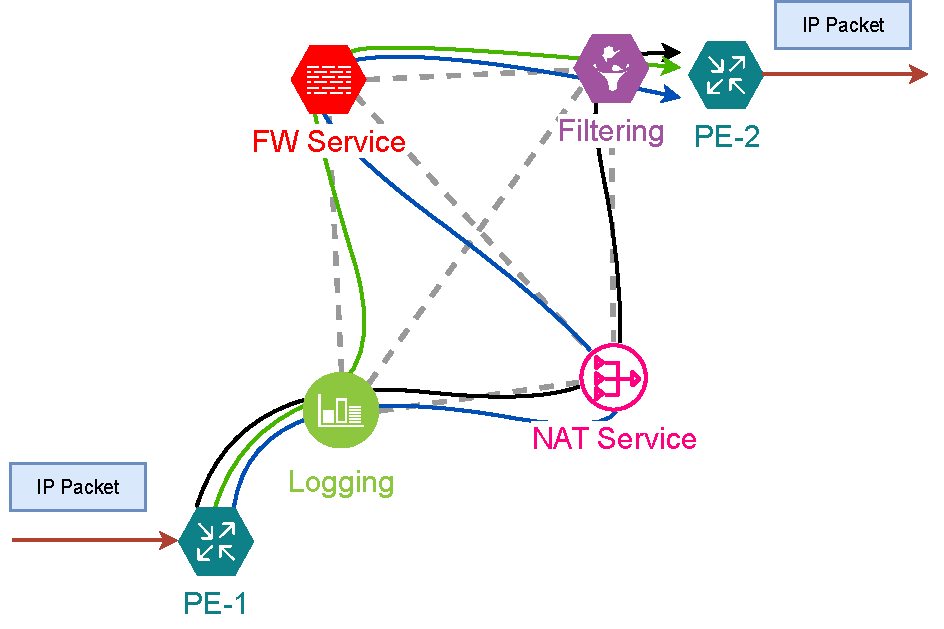
\includegraphics[width=0.95\linewidth]{img/SFC.pdf}
    \caption{SFC Architecture}
    \label{fig:sfc-arc}
\end{figure}

\section{従来のパケットルーティングとトラフィックエンジニアリング}
\label{section:src-rtng}

章\ref*{section:sfc} で述べた通り,SFC を実現するためには,エンドツーエンド通信を提供するために必要な複数の SF を決定,及び順序付けし,それらを介するようにトラフィックを操作する必要がある.
しかし,従来のパケットルーティングでこのようなトラフィック操作を実現することは難しい.

ルータが IP パケットを転送するとき,ルータは自身の持つ経路表を参照する.
この経路表は通常,BGP~\cite{rfc4271} や OSPF~\cite{rfc2328},IS-IS~\cite{rfc1142} などのルーティングプロトコルを通じて交換した経路情報から作成される.
一般的に,多くのルーティングプロトコルでは「経由するノードの数を最小にする経路を最も良いものとする」という基本設計をもとに,オペレータが任意に決定したコスト情報などを含めて最も良い経路を計算する.
このように決定された最も良い経路をベストパスといい,経路表には「ある宛先アドレスを持つパケットは次にどのノードに転送するのがベストパスなのか」が書かれている.
ルータは,自身に接続されているノードやルーティングプロトコルを通じて受け取った経路情報が変更されたとき,その変更を近接ルータに通知し,自身の経路表を更新する.
経路表はオペレータが静的に構築することもできる.しかし,静的に経路を決定してしまうとノードの近接情報が変わるたびにオペレータ自身が設定し直す必要があり,これは手間がかかったりオペレーションミスを誘発したりする問題がある.
そのため,静的な経路設定が利用される場面は限定的である.

図~\ref*{fig:exp-src-rtng} に,あるネットワークのトポロジを示す.
このネットワークにおいて,User-B の通信は青いパスを通るように,User-A から Server に向かう通信は Security appliance を経由させるような経路制御を行いたい.
しかし,Router-B から Router-C までの経路は青いパスを通ると 1 hop だが,Security appliance を通る赤い経路は 2 hop である.
つまり,Router-B から Server までの経路は青いパスの方が経由するノードの数が少ない.
そのため,通常のルーティングプロトコルで経路を学習すると,Router-B の経路表には Server に向かう経路として青いパスがベストパスとして採択される.
ルーティングプロトコルの設定でコストを変更することで赤いパスをベストパスにすることは可能である.
ベストパスを赤いパスに変更すると,User-A の通信については意図通り赤いパスを通るようになる.
しかし,ベストパスを変更してしまうと User-B の通信についても赤いパスを通るようになり,これは意図した経路とならない.

ベストパスによらずに,また特定の通信毎に選択して経路を制御することを,トラフィックステアリング,トラフィックエンジニアリング (TE) という.
TE が可能なパケット転送メカニズムとして,いくつかの候補が存在する.
例えば OpenFlow~\cite{openflow},Network Service Header (NSH)~\cite{rfc8300},MPLS~\cite{rfc3031}などである.

\begin{figure}[t]
    \centering
    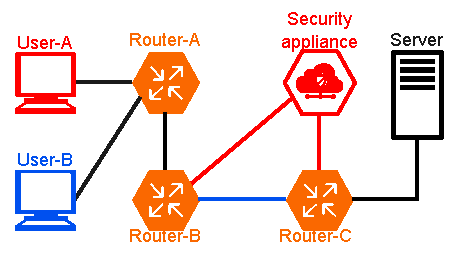
\includegraphics[width=0.95\linewidth]{img/ExplainSrcRtng.pdf}
    \caption{Explain Source Routing}
    \label{fig:exp-src-rtng}
\end{figure}

\subsection*{OpenFlow}
\label{sbsection:openflow}
OpenFlow では,OpenFlow スイッチと呼ばれる OpenFlow に対応した専用の機材をパケットを転送するノードとして使用し,OpenFlow コントローラと呼ばれる専用のマシンが OpenFlow スイッチの経路情報を集中管理する.
OpenFlow のアーキテクチャは一般のパケットルーティングアーキテクチャとは大きく異なる.
一般的なネットワークでは先に挙げた BGP や OSPF などのルーティングプロトコルを利用して経路情報を交換し,経路表を作成する.
そして,ルータは自身が作成した経路表に基づいてパケットを転送する.
対照的に,OpenFlow では BGP や OSPF などのルーティングプロトコルを利用して経路表を作成することはしない.
経路情報は OpenFlow コントローラが集中管理し,OpenFlow コントローラは自身が決定した経路情報を実際にパケットを転送する OpenFlow スイッチへインストールする.
また,OpenFlow では経路表自体も一般的なルーティングで作成されるものとは異なり,OpenFlow で利用される経路表に対応するテーブルのことをフローテーブルという.
OpenFlow のフローテーブルには,宛先の IP アドレスだけではなく,送信元アドレスや通信を受信したポート,独自定義の専用パケットヘッダのフィールドなどもマッチングルールとして含まれる.
これにより,IP 的なベストパスによらずに,かつ同じ宛先であっても別のパスを選択できる.

\subsection*{NSH}
\label{sbsection:nsh}
NSH は,SFC を実現する 1 つの手法として考えられたプロトコルで,NSH と呼ばれるヘッダでパケットをカプセル化する.
OpenFlow が汎用的なパケット転送アーキテクチャとして考案されたのとは対象的に,NSH は SFC を前提として考案された.
NSH で転送されるパケットの構造を図~\ref*{fig:nsh}として示す.
NSH パケットは,大きく分けて 3 のパートに分けられる.
Original Packet は,実際のエンドツーエンドでやり取りするパケットのことを指す.
そのパケットを,NSH でカプセル化している.
NSH の中にはいくつかのフィールドが存在し,その中には SFC の中でどのパスを通過するのか通過するのかや,ユーザ定義のメタデータ,オプショナルなフィールドなどが含まれる.
NSH でカプセル化されたパケットを,更に Transport Encapsulation というヘッダがカプセル化している.
この Transport Encapsulation は特定のフォーマットである必要はなく,GRE,VXLAN などの一般的なトンネリングプロトコルや通常のイーサフレームである.
Transport Encapsulation の目的は,オーバーレイネットワークを通じて適切な SF ノードまでパケットを転送することである.
NSH に対応したノードでは,SF が適用されたパケットに対して,そのパケットの NSH を参照し次の SF のノードを決定する.
次の SF ノードが決まったらそのノードに届くよう,対応する Transport Encapsulation でカプセル化することで TE ができる.
\begin{figure}[t]
    \centering
    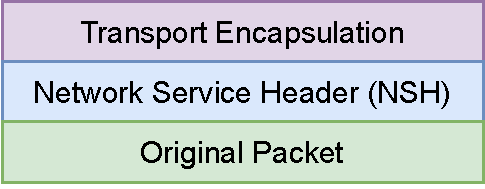
\includegraphics[width=0.95\linewidth]{img/nsh.pdf}
    \caption{Structure of NSH}
    \label{fig:nsh}
\end{figure}

\subsection*{MPLS}
\label{sbsection:mpls}
MPLS とは Multiprotocol Label Switching の略称であり,MPLS ヘッダに含まれるラベル情報に基づいてパケットを転送するプロトコルである.
MPLS ヘッダは Layer 2 ヘッダと Layer 3 ヘッダの間に挿入され,MPLS ヘッダの中にラベル情報を始めとするいくつかのフィールドが埋め込まれる.
MPLS では,宛先の IP アドレスではなく,MPLS ヘッダに含まれるラベル情報を参照してパケットを転送する.
つまり MPLS では,MPLS ヘッダ内に埋め込まれたタグ情報を使ってパケットを転送するため,IP 的なベストパスによらないルールでパケットを転送できる.
また,MPLS は古くから VPN を構成するために用いられてきた一般的なプロトコルである.
そのため,多くのネットワーク機器でサポートされている.
OpenFlow は特別な機器やコントローラが必要であり,NSH も比較的新しいプロトコルで,かつ機能も SFC に特化しているため,NSH をサポートする機材は少ない.
対象的に MPLS は既に多くの機器でサポートされているため,OpenFlow や NSH と比較して導入が容易であるという特徴を持つ.
また,RFC8595~\cite{rfc8595} のように,NSH と MPLS を組み合わせて SFC を実現する手法も提案されている.
このアーキテクチャでは,NSH の Transport Layer として MPLS を利用している.

\section{SRv6}
\label{section:srv6}
先に挙げた技術だけではなく,Segment Routing over IPv6 (SRv6) も TE を適用できる技術の 1 つである.
MPLS が独自のラベルを使って使ってパケットを転送するアーキテクチャであるのに対し,SRv6では MPLS のラベルに対応する概念として IPv6 アドレスを利用する.
SRv6 で利用される識別子はセグメント識別子 (SID) と呼ばれ,各 SID はネットワーク内の特定の場所で実行される特定の機能を表す.
この SID は IPv6 と全く同じフォーマットをしている.
SRv6 では,SRv6ヘッダ (SRH) と呼ばれる IPv6 拡張ヘッダに SID の一連の集合からなるリストを埋め込むことで,ネットワークオペレータやアプリケーションはパケットが通過する中間地点を指定できる.

SRv6 ヘッダには通過するネットワーク上のノードの順番がリストとして埋め込まれ,ルータはそのリストに基づいてパケットを転送する.
図~\ref*{fig:srv6} において,例えば SID リストの要素が \textbf{A,FW,C} である場合,パケットは緑色のパスを通るように転送される.
また,SRv6 はあるパケットが経由するノードを指定できるだけでなく,パケットに対してパケットに対して特定の操作を適用できる.
このようなパケット操作の種類のことを \textbf{SRv6 ビヘイビア} という.
現在 RFC8986~\cite{rfc8986} では 15 種類の End ビヘイビアが定義されている.

\subsection*{SRv6 を利用した layer-3 VPN の構築例と SRv6 によるパケット転送の具体的な動作}
\label{sbsection:srv6-vpn}

SRv6 ビヘイビアを組み合わせることで,layer-3 VPN を構成することもできる~\cite{rfc9252}.
SRv6 を利用した layer-3 VPN の動作を図~\ref*{fig:srv6-vpn} に示す.
図~\ref*{fig:srv6-vpn} \circled{1} において,PE-1 は受信したパケットを SRH でカプセル化する.
このように SRH でパケットをカプセル化する,という操作も SRv6 ではビヘイビアとして定義されており,この操作のことを H.Encaps という.
ここでは,PE-1 は受信したパケットに対して \textbf{A,FW,C} を意味する SID リストを付加したものとする.
このとき,SRv6 でカプセル化されたパケットの宛先アドレスは,内部パケットの宛先アドレスに関わらず,次に到達すべきノードを示す SID である FW Service になる.
PE-1 は H.Encaps で SRH を付加したパケットを Router-A へ送信する.
このとき,パケットは宛先 IPv6 アドレスが Router-A である単なる IPv6 パケットとして扱われる.
PE-1 は自身の持つ経路表を参照し,Router-A へのネクストホップを決定し,パケットを送出する.
図~\ref*{fig:srv6-vpn} \circled{2} は,Router-A が受信したパケットに対して SID を 1 つ進めて FW Service にパケットを転送している様子を示している.
リスト状になっている SID の中でどれが現在有効な SID であるかを指定するために,SRH にはセグメントレフト (segleft) と呼ばれるフィールドが定義されている.
segleft は SID リストのインデックスであり, $(SID の合計)-1$ から始まり,$0$ で終わる.
Router-A は受信した SRv6 パケットの segleft を 1 つデクリメントし,FW Service の SID が次に有効な SID であることを示すようにする.
また,Router-A はパケットの宛先アドレスを新しく有効になった FW Service の SID に書き換える.
このように,segleft を 1 つ進め,宛先アドレスを新たに有効になった SID で書き換える動作のことを End ビヘイビアといい,これも SRv6 ビヘイビアの 1 つである.
End ビヘイビアは SRv6 の中で最も基本的なビヘイビアである.
宛先アドレスを書き換えたあと,Router-A は自身の経路表から新たな宛先アドレス (FW Service の SID) を検索し,ネクストホップへ転送する.
図~\ref*{fig:srv6-vpn} \circled{3} では,\circled{2} と同様に FW Service が End ビヘイビアを実行して segleft デクリメントし,新たに有効になった SID に基づいて Router-C へパケットを転送している.
図~\ref*{fig:srv6-vpn} \circled{4} では,PE-2 が受信したパケットに対して End.DT4 というビヘイビアを実行している.
このビヘイビアは,SRH を取り除き,特定の VRF を参照して SRv6 でカプセル化されていた内部パケットを転送する,という動作を実行する.
End.DT4 により,パケットから SRH は取り除かれ,PE-1 でカプセル化される前のパケットを得ることができる.

\subsection*{SID の構造と構造的な利点}
\label{sbsection:srv6-sid-struct}
先に述べた通り,SID は SRv6 で利用される識別子であり,SRH にはいくつかの SID がリスト状になって含まれる.
図~\ref*{fig:exp-src-rtng} で示されているように,SID は \texttt{LOC:FUNCT:ARG} という 3 つのパートに分かれている.
また,SID は IPv6 アドレスであるため,それら 3 つパートの長さの合計は 128bit である.
\texttt{LOC} はロケータを表す.ロケータとは,ある SID に対応するノードの場所を表す.
\texttt{FUNCT} は SID に関連付けられた SRv6 ビヘイビアの識別であり,\texttt{ARG} はビヘイビアの動作に必要な追加情報をエンコードする領域である.
例えば,End.DT4 では \texttt{ARG} フィールドにはルックアップするべき VRF テーブルを識別するための情報がエンコードされる.

% SRv6 ノードは,宛先 IPv6 アドレスがノードに設定されたローカル SID であるパケットを受信すると,SID に関連付けて事前定義された動作を実行する.
% SRv6 のコンテキストにおいて,SRv6 ノードが実行するパケット操作は End ビヘイビアと称される.
% 現行の RFC8986~\cite{rfc8986} では,15 種類の End ビヘイビアが定義されており,その中で最も基本的なものは End である.
% End ビヘイビアは,受信したパケットの SRH の segleft をデクリメントし,宛先 IPv6 アドレスを次の SID に置換する.
% 続いて,SRv6 ノードは更新された宛先 IPv6 アドレスに基づき,パケットを次のホップに転送する.
% また,RFC8986 では,SID リストを含む SRH でパケットをカプセル化する動作も定義されており,これは Headend ビヘイビアと呼ばれる.
SRv6 の SID は IPv6 アドレスであるため,既存のルーティングプロトコルを用いて SID を経路情報として既存のルーティングプロトコルを利用して広告できる.
SRv6 ビヘイビアは,SID の \texttt{FUNCT} パートで表現される.
しかし,「特定の SRv6 ビヘイビアならば \texttt{FUNCT} パートはこの値である」というようなルールは存在しない.
つまり,SRv6 ビヘイビアの定義は IS-IS の TLV の Type フィールドのようなものとは異なり,ビヘイビアに対応する値は標準化されず,オペレータが自由に決めることができる.
図~\ref*{fig:srv6-vpn} \circled{4} では,Router-C は受信したパケットに対して End.DT4 を実行している.
Router-C は \texttt{LOC:FUNCT:ARG} のフォーマットに従って [Router-C のロケータを示すブロック]:[Router-C 上で End.DT4 として定義されたブロック]:[利用可能な VRF table 番号] を自由に決定し,それを経路情報として周りのノードへ広告する.

SRv6 ビヘイビアが実装されていないネットワーク機器が SRv6 でカプセル化されたパケットを受信した際,その機器は SRv6 パケットを IPv6 パケットとして転送できる.
SRv6 が IPv6 拡張ヘッダを利用したプロトコルであるため,そのパケットは IPv6 パケットとして認識されるからである.
つまり,SRv6 ビヘイビアを実行せず,単にパケットを現在有効な SID へ転送するだけであれば,IPv6 パケットフォワーディングが実装されていれば適切にパケットを転送できる.

% SRv6 ベースのネットワーク構築が可能である.
% 例えば,H.Encaps と End.DT4 はそれぞれヘッドエンドビヘイビア及びエンドビヘイビアに該当し,これら2つのビヘイビアを組み合わせることで layer-3 VPN を構成できる~\cite{rfc9252}.
% H.Encaps は IPv4 または IPv6 パケットを SRH を含んだ IPv6 ヘッダで包み,一方 End.DT4 は SRH でカプセル化されたパケットの外部ヘッダを外す.
% このようにパケットを新たな外部ヘッダで包むことをカプセル化と称し,包まれた外部ヘッダを取り外して内部のパケットを取り出すことをデカプセル化と称す.
% 入口となる SRv6 ノードでは, H.Encaps が出口側 SRv6ノードの End.DT4 SID に対応する IPv6 アドレスを宛先として持つ IPv6 ヘッダで,送信するパケットをカプセル化する.
% 該当パケットは SRv6 ルーティングインフラを通じて,End.DT4 SID の \texttt{LOC} に沿って出口 SRv6 ノードへと転送される.
% SID は IPv6 アドレスであるため,通信の途中の経路ではカプセル化された外側の IPv6 ヘッダの宛先アドレスに基づいてルーティングされる.
% 出口 SRv6 ノードがパケットを受信すると,そのノードは End.DT4 を実行する.
% End.DT4 を実行するとパケットはデカプセル化され,内部パケットは SID の \texttt{ARG} に関連付けられた VRF (Virtual Routing and Forwarding) テーブルに基づいてルーティングされる.

\begin{figure}[t]
    \centering
    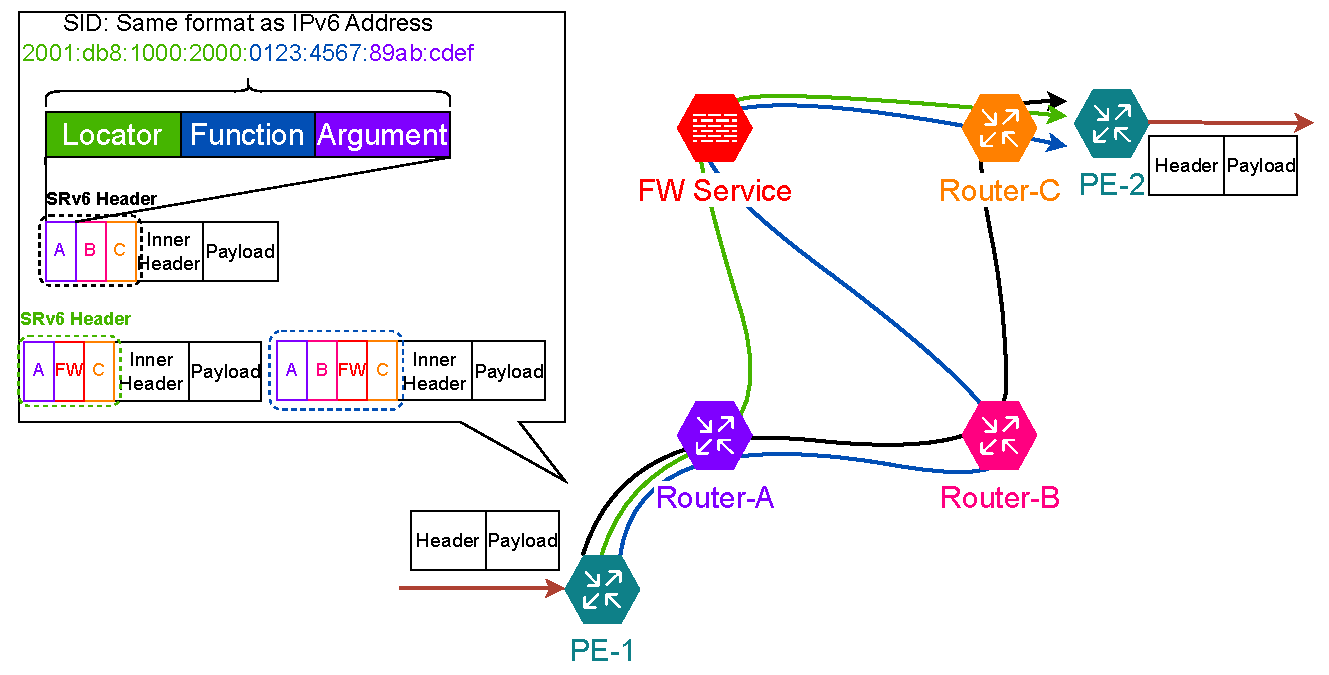
\includegraphics[width=0.95\linewidth]{img/SRv6Arch.pdf}
    \caption{Architecture of SRv6}
    \label{fig:srv6}
\end{figure}

\begin{figure}[t]
    \centering
    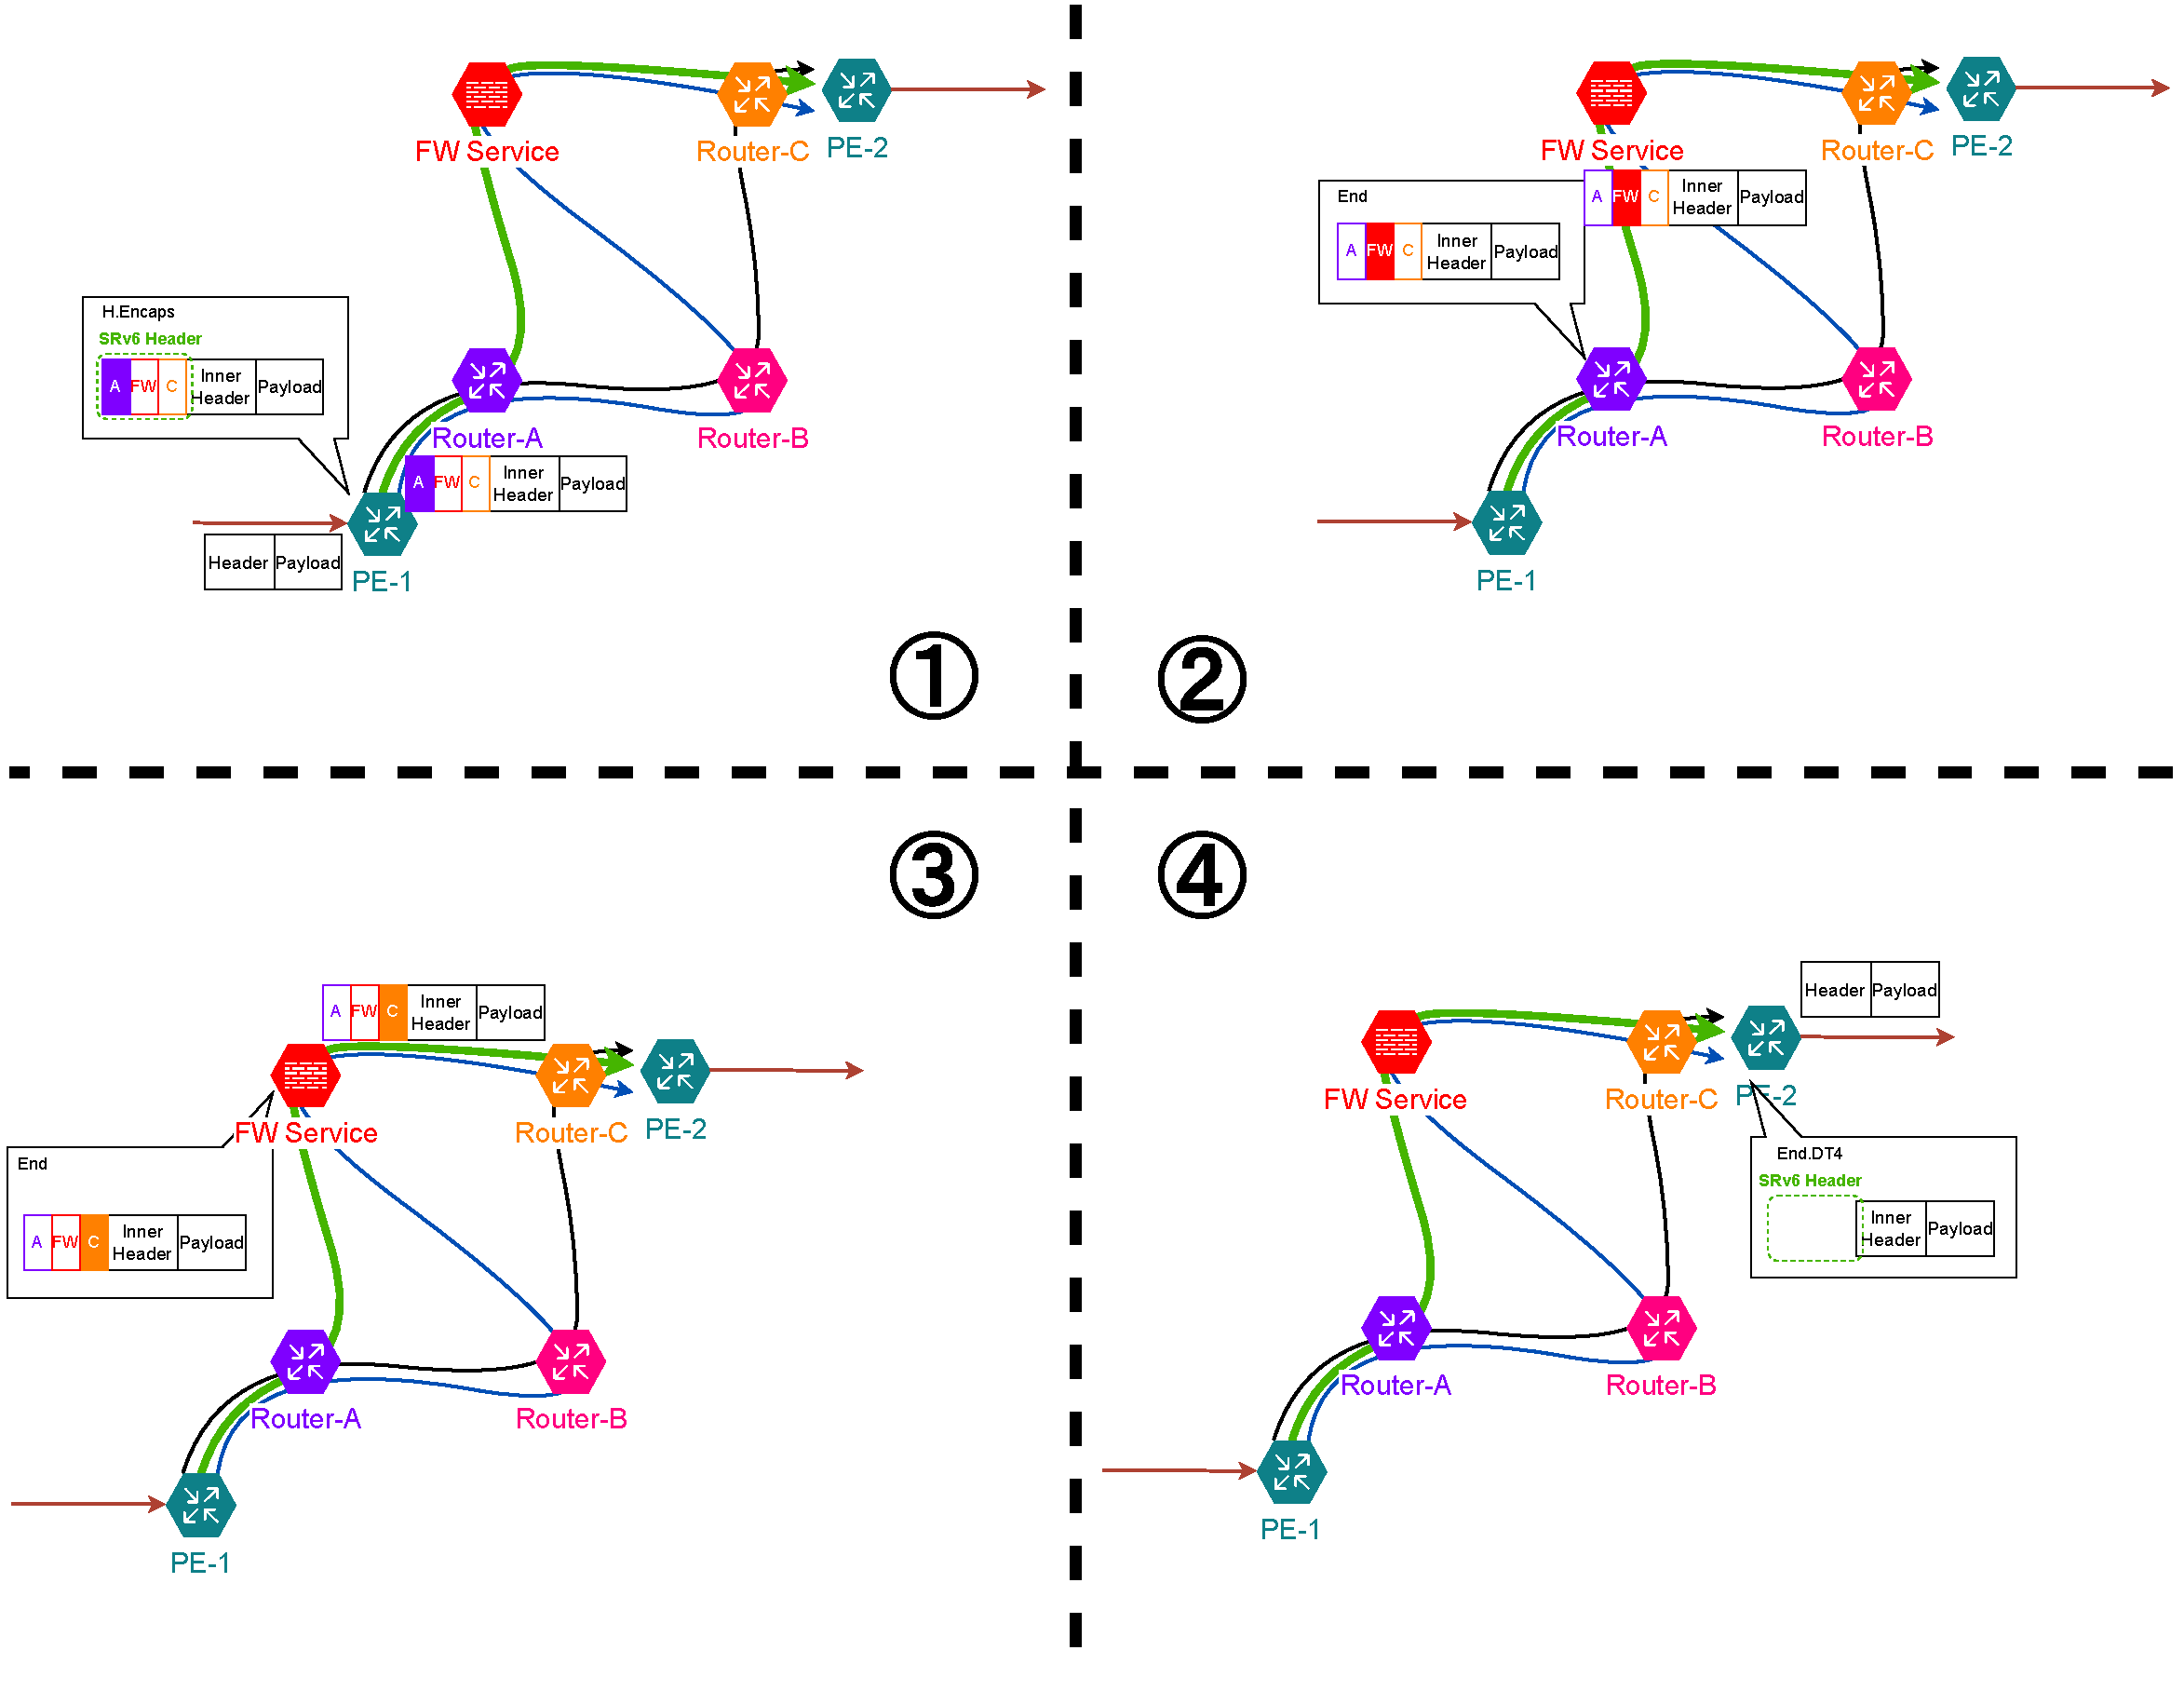
\includegraphics[width=0.95\linewidth]{img/ExplainEndDT4.pdf}
    \caption{layer-3 VPN with SRv6}
    \label{fig:srv6-vpn}
\end{figure}

\section{導入}
\label{section:background}
Service Function Chaining (SFC) は,Software Defined Network (SDN) 及び Network Function Virtualization (NFV) の文脈で研究されているトピックである~\cite{nfv,sfc-on-sdn-nfv-servey,sfc-on-sdn-scenario,imple-sfc-with-openflow}.
SFC では,ネットワーク機能 (NF) を通過する順序や NF のタイプに関する情報を事前に定義し,それらのルールをネットワーク機器に配布する必要がある.
SFC ネットワークを構築するネットワーク機器は,事前に決定されたルールに従って受信したパケットを NF に導く.
パケットを NF へ導くためのルールは,SDN コントローラやルーティングプロトコルによってネットワーク機器に配布される.
ネットワーク機器は IP ルーティング上の最短経路に関係なく,配布された SFC ルールに従ってパケットを転送する次のホップを選択する必要がある.
また,パケットのヘッダにこれらのルールに合致させるための特別な情報を埋め込む手法が取られることもある.
SFC は,クラウドサービスプロバイダ (CSP),アプリケーションサービスプロバイダ (ASP) 及びインターネットサービスプロバイダ (ISP) にとって,現在の静的な環境に代わる柔軟かつ経済的な選択肢を提供する~\cite{survey-on-sfc}.

SFC を実現可能な技術には,いくつかの候補が存在する.
例えば OpenFlow~\cite{openflow},Network Service Header (NSH)~\cite{rfc8300},MPLS~\cite{rfc8595}などである.
これらの技術はどれも,最短経路に関係なく,ルールに基づいて受信したパケットを意図した NF に導く,という要件を満たすことができる.
OpenFlow では,経路情報を管理する中央のコントローラが,実際にパケットを転送する OpenFlow スイッチに対して明示的にパケット転送ルールを設定する.
OpenFlow スイッチは,コントローラによって適切に管理されたルールに従い,パケットを意図した NF に転送する.
OpenFlow のもつこのアーキテクチャは,従来のルーティングプロトコルに基づかない柔軟な経路制御を可能にする.
NSH は Service Path Identifier (SPI) とService Index (SI) によって NF を識別する.
NSH ノードは,パケットに付与された NSH 内の SPI,SI に基づいてパケットを転送する.
NSH は,サービスプレーンと呼ばれる専用のオーバーレイネットワークを作成し,そのオーバレイネットワーク内でサービスを転送する.
このオーバレイネットワークを構築する,というアーキテクチャにより,NSH では基礎となるネットワークトポロジを変更することなくサービス転送を可能にする.
一方,MPLS では,直接 NSH を使用する代わりに,MPLS ラベルスタックを利用する.
このラベルスタックには,パケットが通過すべきノードの順序がホップバイホップで含まれている.
ラベルスタック内で表現されるノードはルータだけでなく,NF も含まれるため,そのラベルスタックに基づいてパケットを転送する事で SFC を実現できる.
このアプローチもまた,基礎となるネットワークトポロジを変更せずに SFC を実現するために必要な,最短経路によらないパケット転送を達成する.

Segment Routing (SR),特に Segment Routing over IPv6 (SRv6) もまた,SFCを実装するために使用される技術の1つである.
SR では,リンク,ノード,サービスといったネットワーク内の各エンティティを\textbf{セグメント}として表現する.
SRv6 パケットのヘッダ (SRH) には,セグメントリストと呼ばれる,そのパケットが通過すべきセグメントの順序を示したリストが含まれている.
SRv6 では,セグメントを識別するための ID (SID) として,IPv6 アドレスを使用する.
言い換えれば,SRv6 は IPv6 ルーティングインフラをその基盤として利用し,SRH 内で定義された順序に従って,任意のセグメントを経由してパケットを転送する.
SRv6 は,NF が実行されるノードをセグメントとして表現し,SID を割り当て,任意の順序で NF を通過するようにパケットを転送することで SFC を実現する.

SRv6 では,NF を SID で表し,セグメントリストに基づいて適切にパケットを転送をすることで,SRv6 を基盤とした SFC ネットワークを実現できる.
しかし,SRv6 レイヤよりも上位にある NF の振る舞いと,基盤となる IPv6 ルーティングインフラをどのように統合するかは明確でない.
例えば,IPv4パケットの Network Address Translation (NAT) を SRv6 ネットワーク内の NF として考慮する場合を考える.
SRv6 ネットワーク内において,IPv4パケットは,SR Header (SRH) を含む外部 IPv6 ヘッダでカプセル化される.
NF で動作する NAT の実装が SRv6 に対応していない場合,SR プロキシ~\cite{ietf-spring-sr-service-programming-08}が必要となり,ネットワーク構成や運用における複雑さが増加してしまう~\cite{draft-scexp}.
実装が内部パケットへの NAT と SRv6 に則した転送動作を同時に実行できる場合,それはレイヤバイオレーションとなる. 
Linux には,SERA~\cite{sera} という iptables を拡張したファイアウォールアプリケーションが存在する.
SERA は SRH でカプセル化されたパケットについて,カプセル化された内部パケットのヘッダ情報にマッチする iptables のフィルタールールを適用できる.
SRv6 での基本的な転送動作として,End と呼ばれる動作がある.
SERA は iptables を拡張することで,この End 動作を処理する機能も実装されている.
ただし,既にLinux カーネルには IPv6 ルーティング,及び SRv6 End 動作に関する処理が実装されている.
SERA は,Linux カーネルに実装されている SRv6 機能を使わずに,独自に改良した iptables アクションによって End 動作を処理する.
つまり,SERA は Linux カーネル内で統合されている IPv6 ルーティングインフラと SRv6 処理機能を使わずに,独自に拡張した iptables によって SRv6 とフィルタリングサービスとしての NF を統合している.

本論文では,既存の netfilter ベースアプリケーションの実装を変更することなく SRv6 対応 NF として扱えるようにする,End.AN.NF 提案する.
End.AN.NF は Linux netfilter を NF として扱えるようにしつつ,Linux に実装されている IPv6 ルーティングインフラを活用する.
End.AN.NF は受信した SRv6 内部パケットに対して,netfilter のフックポイントを透過的するように設計されている.
本論文では End.AN.NF を Linux カーネル上で実装し,スループットとレイテンシを評価した.
評価の結果,End.AN.NF は End.DT 4と H.Encaps の組み合わせによる SRv6 内部パケットへの netfilter 適用と比較し て27\% 高いスループットと 3.0 マイクロ秒低いレイテンシを実現した.
さらに,End.AN.NFのレイテンシは,End.DT4とH.Encapsの組み合わせよりも3.0マイクロ秒低い.
また,End.AN.NFのレイテンシはマイクロ秒解像度でEnd動作と同じである.

\section{本論文の目的と構成}
本論文における以降の構成は次の通りである.
\ref*{chap:introduction}章では,本論文の構成,及び本論文の概要を述べる.
\ref*{chap:related_works}章では,サービスファンクションチェイニングに関する前提知識,及びそれを実現する技術について解説し,本論文の概要について述べる.
\ref*{chap:design_and_impl}章では,本論文の提案する新たな SRv6 End behavior である End.AN.NF についての詳細な動作,及び実装について述べる.
\ref*{chap:evaluation}章では,実装した End.AN.NF について,レイテンシ及びスループットの性能を特定のを変化させながら性能の計測する.
\ref*{chap:conclusion}章では,本研究における結論と今後の展望について述べ,End.AN.NF に必要なネットワーク制御プレーンについて検討する.
\chapter{背景と問題提起}
\label{chap:related_works}
% 本章では,Service Function Chaining (SFC),及びそれを実現する技術について解説する.
% SFC を実現するための技術は複数存在する.
% 本論文では,複数ある技術の中で Segment Routing over IPv6 (SRv6) における SFC を前提としているため,SRv6 の概念やその知識についても解説する.
章~\ref*{chap:introduction} では,SFC の概念と SFC を実現するための要件を満たせるいくつかのプロトコルを説明し,近年特に注目されている SRv6 について説明した.
その知識を踏まえた上で,本章では背景と本研究で解決するべき問題を提起する.

\section{Linux と netfilter}
\label{section:linux-and-netfilter}
SFC をデプロイする上で,SF を動作させる環境として Linux を選択することは有用である.
章~\ref*{section:sfc} で述べたように,SFC 環境では SF を汎用サーバや仮想マシン,コンテナの中にデプロイすることが一般的になっている.
Linux 上で任意のアプリケーションを開発して,そのバイナリを動作させることは容易であり,開発に必要な基盤や情報も十分に整っている.
更に Linux kernel はコンテナメカニズムもサポートしており,SF アプリケーションをコンテナの中で動作させることも可能である.
また,Linux kernel にはパケットフォワーディング機能が実装されている.
IPv4 パケットや IPv6 パケットの転送はもちろん,MPLS や VXLAN,更にはいくつかの SRv6 ビヘイビアも実装されている.
SRv6 では既存のルーティングプロトコルを使って SID を経路情報として他のルータへ広告することができる.
Linux には FRR~\cite{frr} や gobgp~\cite{gobgp} などのルーティングソフトウェア実装が存在し,これらを利用して SID を広告できる.

Linux kernel には netfilter~\cite*{netfilter} と呼ばれるパケット処理フレームも実装されており,これは SF アプリケーションを開発するのに有用である.
netfilter は,パケットのフィルタリングやロギング,NAT,NAPT,やその他のパケットマングリングを可能にするフレームワークである.
netfilter は,iptables や nftables といったパケット処理アプリケーションの内部の実装に使われている.
iptables や nftables といった,netfilter を基盤として実装されたアプリケーションのことを,本論文では netfilter-based アプリケーションと呼ぶ.
netfilter-based アプリケーションの例として,iptables や nftables 以外にも,conntract-tools\cite{conntract-tools} や snort\cite{snort} といったアプリケーションも存在する.

netfilter の仕組みを使うと,任意のカーネルモジュールは Linux kernel のネットワークスタック上で定義された特定の場所に場所にコールバック関数を設定できる.
カーネルモジュールとは,Linux カーネルのソースコードそのものを書き換えず,かつマシンの再起動を必要としない Linux kernel の機能を拡張するプログラムのことである.
一般的なユーザ定義のアプリケーションはユーザ空間で動作するため,カーネル空間で特定のプログラムを実行することはできない.
しかし,カーネルモジュールとして動作するプログラムは,カーネル空間で動作する.
つまり,開発者はカーネルモジュールを開発することで Linux kernel に機能を追加することができる.

netfilter によってコールバック関数を設定できるポイントの一覧を,図~\ref*{fig:nf-hooks} として示す.
なお,この図は wiki.nftables.org より引用した図である.
図~\ref*{fig:nf-hooks} から読み取れるように,netfilter は Linux のネットワークスタックの様々な場所にコールバック関数を設定することができる.
これらの netfilter がコールバック関数を設定できるポイントを,netfilter フックポイント,または単にフックポイントという.
いくつかのフックポイントは,現在処理しているパケットの宛先が自分自身かどうかによって通過するかしないかが変わる.
例えば,IP レイヤに存在するフックポイントでは,パケットの宛先アドレスが自分であれば Input Hook を通過するが,そうでない場合は Forward Hook を通過する.
Forward Hook にのみ特定のパケットをフィルタリングするコールバック関数を登録することで,自身宛のパケットはフィルタリングをかけないが,転送するパケットにのみフィルタリングを適用する,という使い方ができる.

\begin{figure}[t]
    \centering
    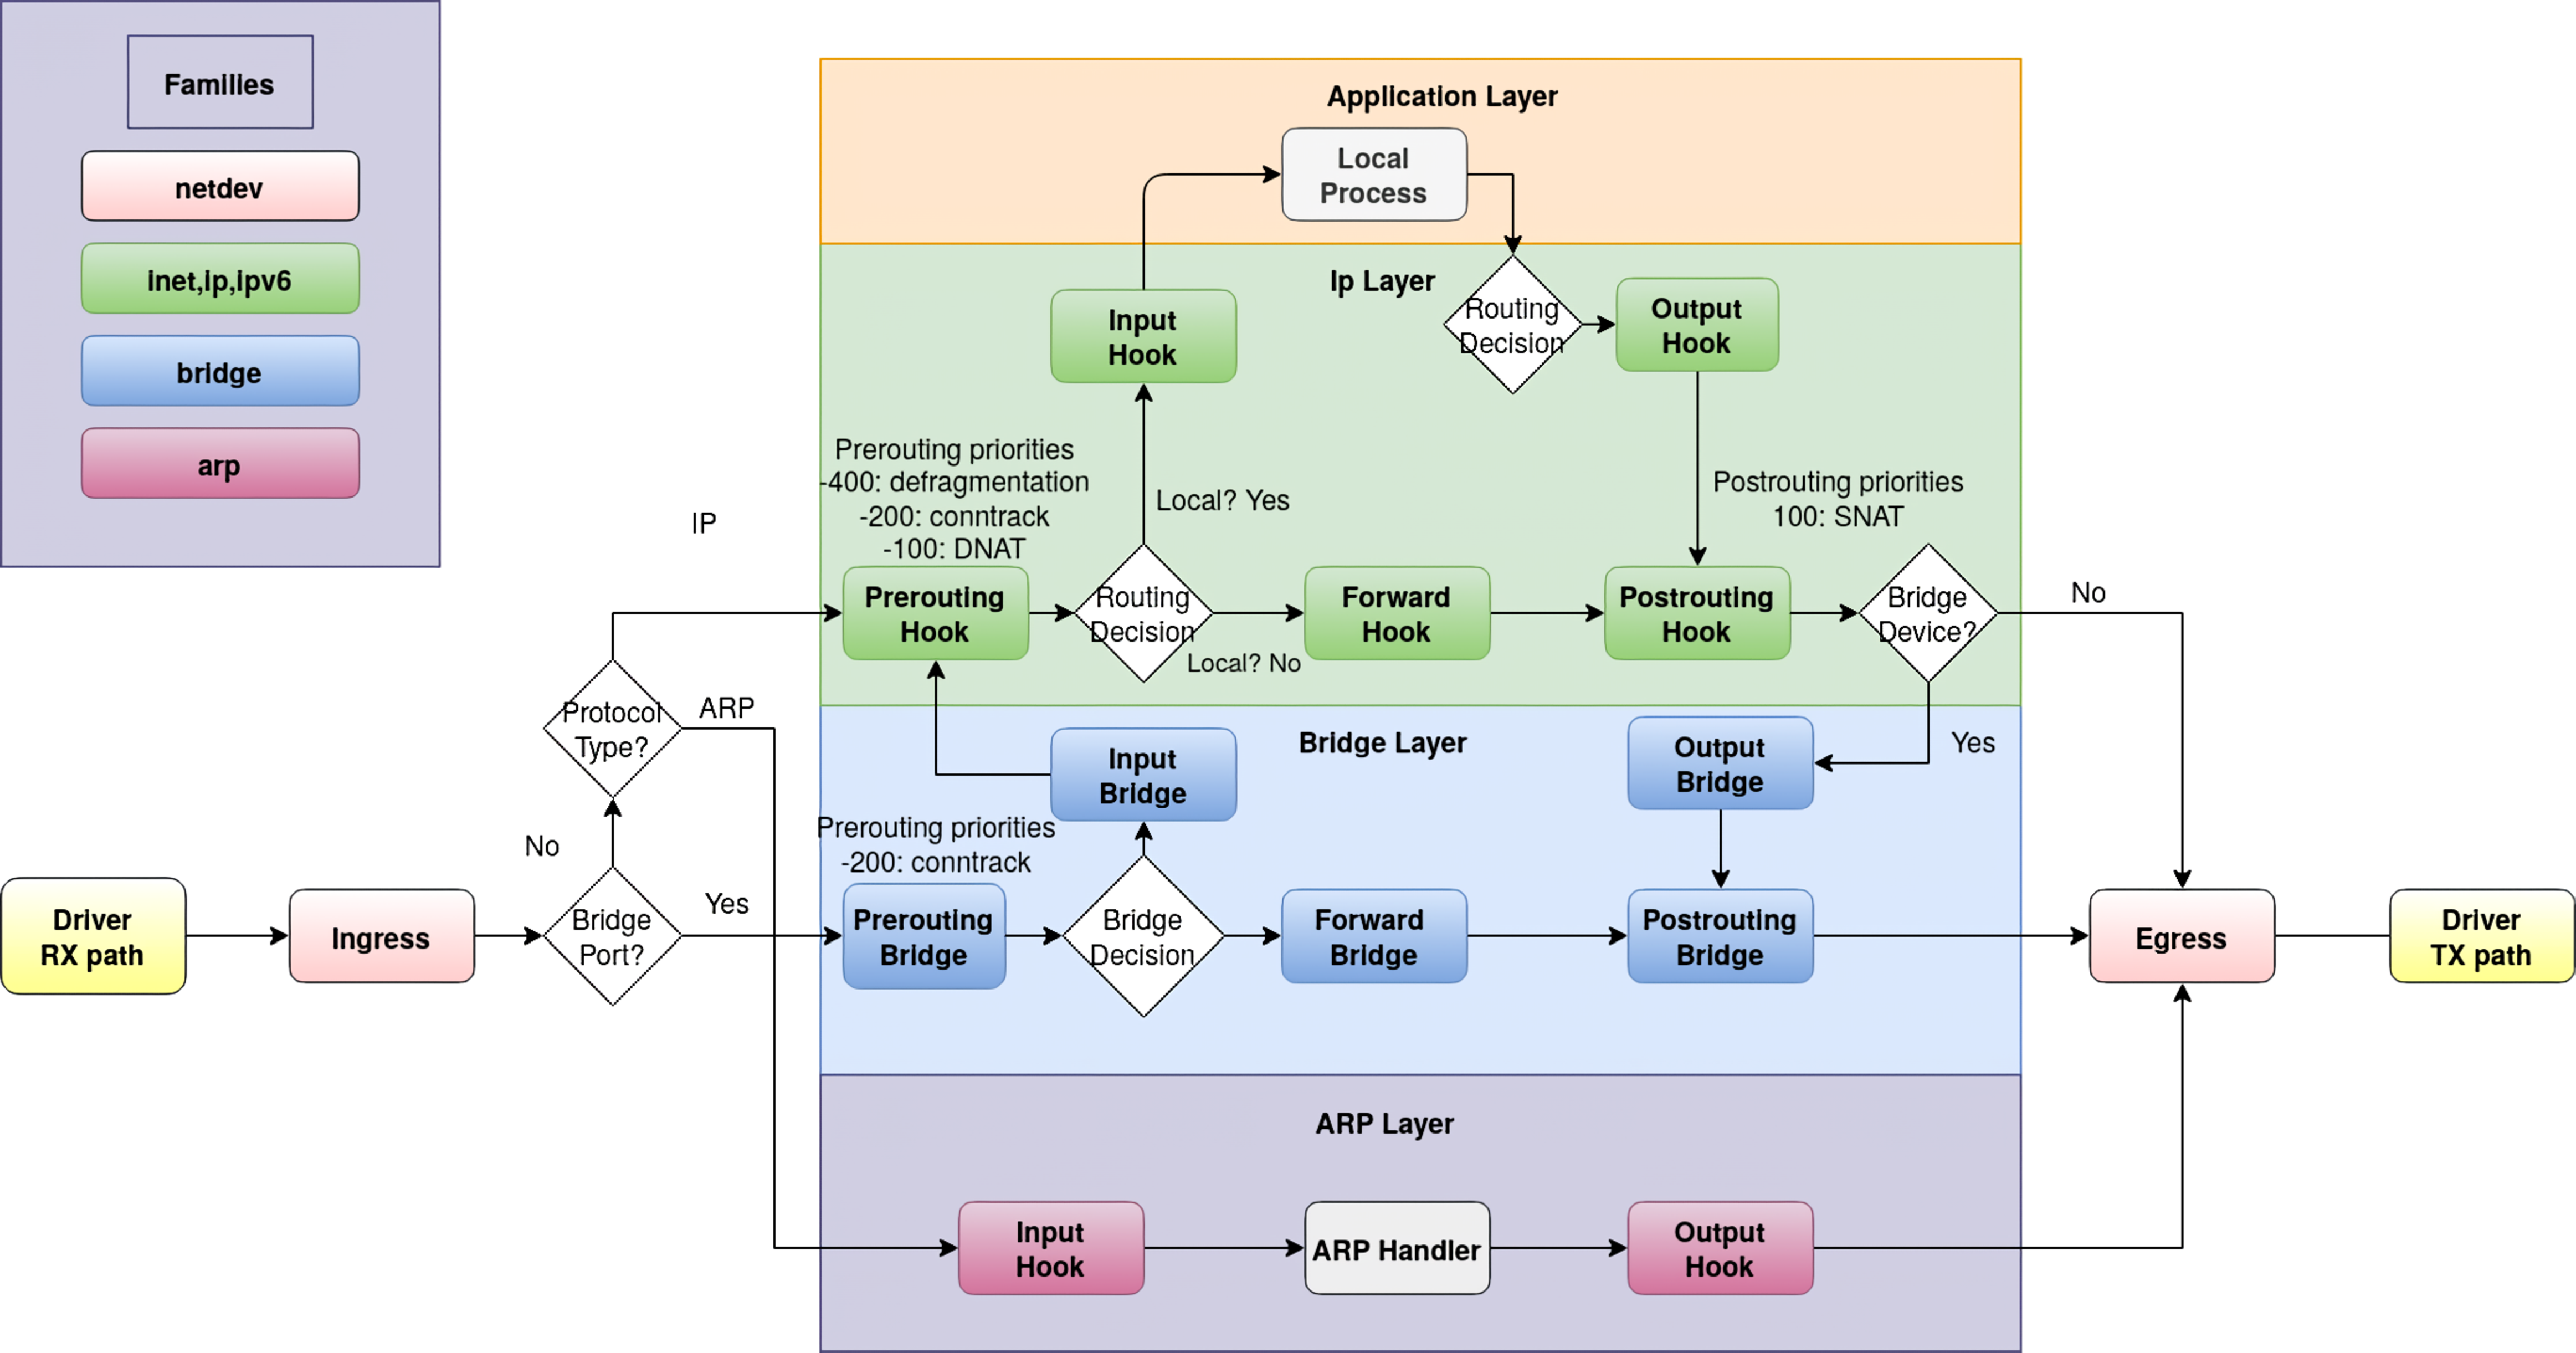
\includegraphics[width=0.95\linewidth]{img/nf-hooks.pdf}
    \caption{netfilter hook points (wiki.nftables.org より引用~\cite{nf-hooks})}
    \label{fig:nf-hooks}
\end{figure}

\section{SRv6 と SF としての netfilter 統合手法}
\label{section:netfilter-as-nf}
Linux netfilter と SRv6 を利用して SFC をデプロイすることは有用な手法であるように思えるが,実際には問題が存在する.
章~\ref*{section:linux-and-netfilter}で述べたように,Linux kernel には SRv6 の機能が実装されており,netfilter は SF アプリケーションの開発に有用である.
しかし,netfilter は SRH でカプセル化された内部のパケットに対して netfilter hook point を適用できない.
これは転送するパケットのソースアドレスを書き換える NAT 操作を SRv6 パケットの内部に適用しようとしても,SRH でカプセル化されているために通常のパケットと同じ操作では NAT を適用することができないからである.
つまり,一般的な IPv4 パケットに対して特定の操作を行うために実装された netfilter-based アプリケーションを SRv6 の内部 IPv4 パケットに対して適用する事はできない.

SRv6 に対応していない SF アプリケーションのことを,SR-unaware アプリケーションといい,対照的に SRv6 に対応している SF アプリケーションのことを SR-aware アプリケーションという.
SR-unaware アプリケーションを SRv6 環境で SF として利用する方法はいくつか存在する.以降では,3 つの手法について解説する.

\subsection*{アプリケーションの実装を変更する手法}
\label{sbsection:change-impl}
最も単純な方法は,アプリケーション自体の実装を変更し,SR-aware アプリケーションにすることである.
SERA~\cite{sera} は,Linux iptables に統合された SR-aware アプリケーションの実装である.
SERA は Linux iptables を拡張し,SRH のフィールドと iptables のルールをマッチさせて,ファイアウォール用のフィルタリングルールを適用する.
また,SERA は SRH でカプセル化された内部の IPv4 パケットに対してファイアウォールルールを適用する事もできる.
更に SERA は,SRv6 End ビヘイビアのように,パケットを次の SID に転送する機能も持つ.
しかし,SERA は iptables の拡張であるため,その他の netfilter-based アプリケーションを SR-aware にすることはできない.
SERA のような手法で netfilter-based アプリケーションを SR-aware にするためには,アプリケーション毎にその実装を変える必要がある.
また,SERA の採用した iptables を拡張するというデザインは,SERA に関連する SID を既存のルーティングインフラに統合することを困難にしている.
iptables 内のフィルタリングルールとして利用するための SID の情報は,\ref*{section:srv6}章で解説した layer-3 VPN の例とは異なり,既存のルーティングプロトコルを通じて広告することはできない.

\subsection*{SR-proxy を利用する手法}
\label{sbsection:use-sr-proxy}
もう 1 つの方法は,SR-proxy と呼ばれる手法を適用することである.
SR-Proxy の概念図を図~\ref*{fig:sr-proxy} として示す.
図~\ref*{fig:sr-proxy} において,Router-B が SR-proxy を適用するノードである.
Router-B は,Router-A から受信した SRv6 パケットの SRH を一度取り外し,その状態をキャッシュしておく.
Router-B は,取り外して得られた SRv6 の内部パケットを FW ノードへ送信する.
FW ノードが受信するパケットは SRH でカプセル化されてない一般的な IP パケットであるため,FW ノードは受信したパケットを一般的な IP パケットとして解釈し,FW サービスを適用する.
FW ノードは,FW サービスを適用したパケットを再び Router-B に送り返す.
Router-B は FW サービスから受け取った非 SRv6 パケットを,キャッシュしておいた SRH で再びカプセル化する.
Router-B は自身が再度カプセル化した SRv6 パケットを,次の転送先である Router-C へ送信する.

SR-Proxy を利用する方法は,汎用性が高い.
SR-Proxy を実行するノードが SRH を取り外して SF ノードにパケットを転送するため,SF アプリケーションは SRH の存在を意識する必要がない.
この手法であれば,iptables に限らず,あらゆる netfilter-based アプリケーションを SFC 中の SF として扱うことができる.

また,SR-Proxy は SRv6 のビヘイビアとしても提案されており~\cite{filsfils-spring-srv6-interop-02},End.AS や End.AD や End.AM と呼ばれるビヘイビアがそれに該当する.
これらは SRv6 ビヘイビアであるため,それら SID は IPv6 アドレスとして表現され,既存のルーティングプロトコルを使ってそれらの SID を広告することができる.
2024 年 1 月現在,End.AD や End.AM は Linux kernel のメインライン上では実装されておらず,これらの実装はワークインプログレス状態である.
Linux で動作する SR-Proxy として,SRv6 ビヘイビア以外の実装も提案されている~\cite{sfc-proxy-bpf,sfc-with-leg-vnf,afxdp-for-srv6}.

しかし,SR-Proxy を利用する方法には,SERA のような SR-aware アプリケーションには存在しないオーバーヘッドが存在する.
それは,SR-Proxy が一度 SRv6 パケットから SRH をデカプセル化する際に生じるオーバヘッド,一度外部ノードに転送し,SF 適用後に再度受信するオーバーヘッド,そして受信したパケットを再度同じ SRH でカプセル化するオーバーヘッドである.

また,SR-Proxy は根本的にネットワークにさらなる複雑さをもたらす.
SR-Proxy は SF から返されるパケットに付加する適切な SID リストを決定する必要がある.
SF から返される内部パケットは任意の宛先と送信元を持つ可能性があるため,SR プロキシが付けるべき SID リストは内部パケットによって異なる可能性がある.
つまり,SRプロキシは適切な SID リストを決定するための独自のメカニズムを実装する必要がある.
例えば,静的な SID リストをアタッチする End.AS か,プロキシの内部で状態をキャッシュする必要がある~\cite{sfc-proxy-bpf} .
さらに,SR プロキシをデプロイするためにはいくつかの問題が存在する.
例えば,特定の SR-Proxy タイプと共存できないサービスのタイプがあったり,サービスの有効性を検出する必要や SR-Proxy が送信する先の SF に関する SID 広告の問題など~\cite{draft-scexp}が既にインターネットドラフトとして挙げらている.

\begin{figure}[t]
    \centering
    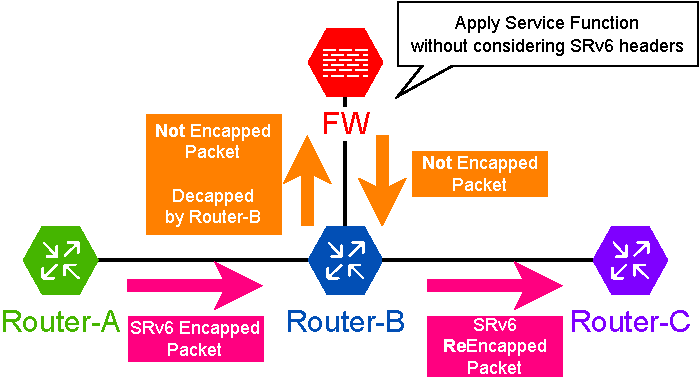
\includegraphics[width=0.95\linewidth]{img/SR-proxy.pdf}
    \caption{SR-proxy Architecture}
    \label{fig:sr-proxy}
\end{figure}

%%%
% \ref*{section:srv6}章で示した End.DT4 及び H.Encaps は,パケットをカプセル化,及びデカプセル化するビヘイビアである.
% 一方で,いくつかのビヘイビアのもつ機能はパケットのカプセル化,及びデカプセル化に限定されていない.
% SRv6 では,パケットに適用される NF (Network Function) も SID で表現可能である.
% NF がトランジットパケットに対して,segleft をデクリメントし,宛先 IPv6 アドレスを次の SID で更新する End ビヘイビアとしての動作をしながらネットワークサービスを適用する場合,その NF は SR-Aware ファンクションと呼ばれる.

% SR-Aware ファンクションと対照的に,従来の SR-unaware NF を SRv6 ベースの SFC に統合するための様々な方法論が提案されている.
% SR プロキシ~\cite{ietf-spring-sr-service-programming-08} は,SR-unaware NF を SRv6 ネットワークに接続するための重要なコンポーネントである.
% SR プロキシは ローカル SID 宛のパケットを受信し,SRH を持たないインナーパケットを関連する NF に渡した後,NF から返されたパケットに適切な SRH を再度付加し,次の SID にパケットを転送する.
% Linux における SR プロキシの実装もいくつか提案されている~\cite{sfc-proxy-bpf,sfc-with-leg-vnf,afxdp-for-srv6}.
% しかし,SR プロキシは根本的にネットワークにさらなる複雑さをもたらす.
% 例えば,SR プロキシは NF から返されるパケットに付加する適切な SID リストを決定する必要がある.
% 内部パケットは任意の宛先と送信元を持つ可能性があり,そのため SR プロキシが付けるべき SID リストは内部パケットによって異なる可能性がある.
% SRプロキシは,適切なSIDリストを決定するための独自のメカニズムを実装する必要がある.
% 例えば,静的な SID リストをアタッチする End.AS か,プロキシの内部で状態をキャッシュする必要がある~\cite{sfc-proxy-bpf} .
% さらに,SR プロキシをデプロイするためにはいくつかの問題が存在する.
% 例えば特定の SR プロキシタイプと共存できないサービスのタイプ,サービスの有効性の検出,SR プロキシの背後のサービスに対する SID 広告の問題など~\cite{draft-scexp}が既にインターネットドラフトとして挙げらている.


% \textbf{[この段落では End.eBPF について述べる]}
% \begin{itemize}
%     \item eBFP とはなにか
%     \begin{itemize}
%         \item eBPF を使って NF を作ることができる 
%         \item 最近では LKM に変わって Linux kernel を拡張する方法としての側面に注目が集まっている
%         \item eBPF は Virtual Machine で動作するものの Linux kernel に依存する機能も多い
%     \end{itemize}
%     \item End.eBPF とはなにか
%     \item eBPF に対して,本研究では netfilter を NF に統合することを目的としている
%     \begin{itemize}
%         \item ここで Linux kernel に依存する End ビヘイビアを提案することの妥当性を述べる
%     \end{itemize}
% \end{itemize}

\section{問題提起}
\label{section:prob}
現在,Linux の持つ SRv6・IPv6 ルーティングインフラストラクチャを活用しながら Linux カーネルに実装されている netfilter という多機能なパケット処理機能 を NF として利用する手法は,確立されていない.
現在提案されている手法では,Linux の持つ IPv6 ルーティングインフラストラクチャを活用した SR-aware アプリケーションをシンプルに汎用的に実現することは難しい.
また,Linux カーネルには netfilter という多機能なパケット処理機能が実装されているものの,SRv6 上で netfilter を直接 NF として扱う方法も確立されていない.
SRv6 は SF を SID として表すことで SFC を実現可能なアーキテクチャであるものの,SID として表現された SRv6 上のノードとしての SF と,実際のアプリケーションとしての SF を統合するの方法は自明ではない.
セクション~\ref*{sbsection:use-sr-proxy}で述べた SR-Proxy を利用する方法では,SR プロキシを導入することで生まれるオーバヘッドや運用上の問題が指摘されている.
また,SRH でカプセル化されているパケットに対して,パケットをカプセル化したまま netfilter 自体を適用する手法も確立されていない.
本論文では,Linux netfilter を SRv6 を使って構築された SFC 上の SF として活用するための手法を提案する.

\chapter{設計と実装}
\label{chap:design_and_impl}
本章では,前提となる Linux カーネルにおけるパケットフォワーディング処理,netfilter に関する知識を解説し,本論文の提案手法についての設計と実装について述べる.
\section{Linux カーネルにおけるパケットフォワーディング}
\textbf{[Linux カーネルにおけるパケットフォワーディングの流れや,その実装について説明する.]}

\section{設計}
SR-Aware NF の新しい実装として,Linux のルーティングインフラに netfilter によるパケットのフィルタリングとマングリング機能を統合した SRv6 End ビヘイビアである End.AN.NF を提案する.
End.AN.NF は,End behavior of SR-Aware Native function for NetFilter の略である.
End.AN.NF の実装は,Linux カーネルの IPv6 ルーティングスタックを活用するように設計されている.
End.AN.NF の SID は IPv6 アドレスとして表現され,Linux 上では IPv6 ルーティングテーブルエントリとして扱われる.
End.AN.NF を示す SID は,通常の IPv6 経路として既存のルーティングプロトコル,及びその実装を介して他のノードに透過的に広告される.
さらに,End.AN.NF では,SRv6 でカプセル化されたインナーパケットに対して,netfilter のルールを適用できる.
End.AN.NF は,nftables\cite{nftables} や iptables~\cite{iptables} を介して設定されたトラフィックに対する選択的なパケット破棄や NAT の適用などを SRH でカプセル化された内部のパケットに対して適用できる.
また,nftables や iptables に限らず,その他の netfilter ベースのアプリケーションについても,それらの実装を変更することなく SR-Aware NF として使用可能にする.

Netfilterは,Linuxのレイヤ3パケット転送フローに3つのフックポイントを持ち,異なるタイミングでパケットに netfilter ルールを適用する.
図\ref*{fig:hooks} は,トランジットパケットに適用される netfilter のフックのフローを示している.
受信したあるパケットに対して End.AN.NF が動作する際,そのパケットは 2 段階の netfilter フックが適用される.
1つ目の適用では,SRH を含む外部 IPv6 ヘッダのついたカプセル化されたパケットに対して,その外部 IPv6 ヘッダをターゲットにして実行される.
2つ目の適用では,SRH を含まない,カプセル化された内部パケットの IP ヘッダをターゲットにして実行される.
まず,End.AN.NF を実装した Linux ベースの SRv6 ノードが IPv6 パケットを受信すると,そのカーネルは受信したパケットに prerouting フックを適用し,通常通り宛先 IPv6 アドレスの最長プレフィックスマッチングを行う.
宛先アドレスがローカルの End.AN.NF の SID である場合,カーネルはパケットを End.AN.NF の実装に渡し,そうでない場合,カーネルは forward フックと postrouting フックを適用しながら,IPv6 パケットを対応するネクストホップに転送する.
一方,End.AN.NF は,SRHでカプセル化されたインナーパケットに対して,再度,prerouting フック,forward フック,及び postrouting フックを適用する.
End.AN.NF の段階で netfilter が適用されている間,SRH は End.AN.NF によって隠されるので,netfilter は SRH の処理を考慮する必要がない.
End.AN.NF が終了すると,外部 IPv6 ヘッダの宛先アドレスは次の SID に置き換えられ,カプセル化されたパケットは Linux の IPv6 パケットフォワーディングプロセスにおける通常の転送パスに戻る.

End.AN.NF は,パケットをマーキングするために SID の \texttt{ARG} フィールドを利用する.
ARG は SID の下位ビットである~\cite{rfc8986}.
SRv6 の仕様では,ある End ビヘイビアがその End ビヘイビア固有の用途で \texttt{ARG} を利用することを許可している.
End.AN.NF では,SID の ARG がマークとして Linux カーネル空間におけるパケットバッファに付加される.
netfilter ベースのアプリケーションは,パケットバッファ上のマークを照合することで,適用するルールを変更することができる.
したがって,オペレータが,単一の End.AN.NF SID しか定義されていない場合であっても,NF は ARG に基づいてトラフィックのルールを調整することが可能である.

アルゴリズム~\ref*{alg:end-an-nf} は,End.AN.NF がパケットを netfilter のフックポイントに渡す方法を示した擬似コードである.
まず,End.AN.NF は,ARG の長さがこの End.AN.NF SID に指定されている場合,受信したパケットの宛先アドレスから ARG 値を抽出する.
抽出された ARG 値は,マークとしてパケットバッファに付加される.
次に,End.AN.NF はパケットバッファの先頭を外側の SRH から内側のパケットに切り替え,バッファを netfilter フックに渡す.
フックにインストールされたルールが内側のパケットに適用された後,End.AN.NF は,パケットバッファの先頭を内側のパケットから外側の SRH に復元し,パケットを次のプロセスに渡す.
この手順は,図~\ref*{fig:hooks} の赤い長方形で示した3つのフックポイント,prerouting,forward,postrouting に対してそれぞれ適用する.

Linux カーネルは,End ビヘイビアを関数の SID を宛先とするルーティングテーブルエントリとして実装している.
このメカニズムは seg6local と呼ばれる.
End.AN.NF は End ビヘイビアの1つであるため,その実装も seg6local を利用している.
図~\ref*{fig:show-route} に示すように,カーネルは他の End ビヘイビアと同様に End.AN.NF を表す SID をルーティングテーブルエントリとして扱っていることが確認できる.
ルーティングソフトウェアや iproute2 を用いて SID をルーティングテーブルエントリとして追加すると,従来のルーティングプロトコルを用いてカーネルのルーティングテーブルにインストールされた経路を広告することが可能となる.
実際に FRRouting~\cite{frr} を使用し,カーネル内の End.AN.NF に関連付けられた SID を BGP 経由で他のルータに IPv6 経路として広告できることを確認した.
End.AN.NF のアーキテクチャは,ルーティング制御に既存のルーティングプロトコルを使用できるため,既存の NF との互換性が高い.
このアーキテクチャは,Linux netfilter を用いた SR-Aware NF の実現方法の一つである.

\begin{figure}[t]
    \centering
    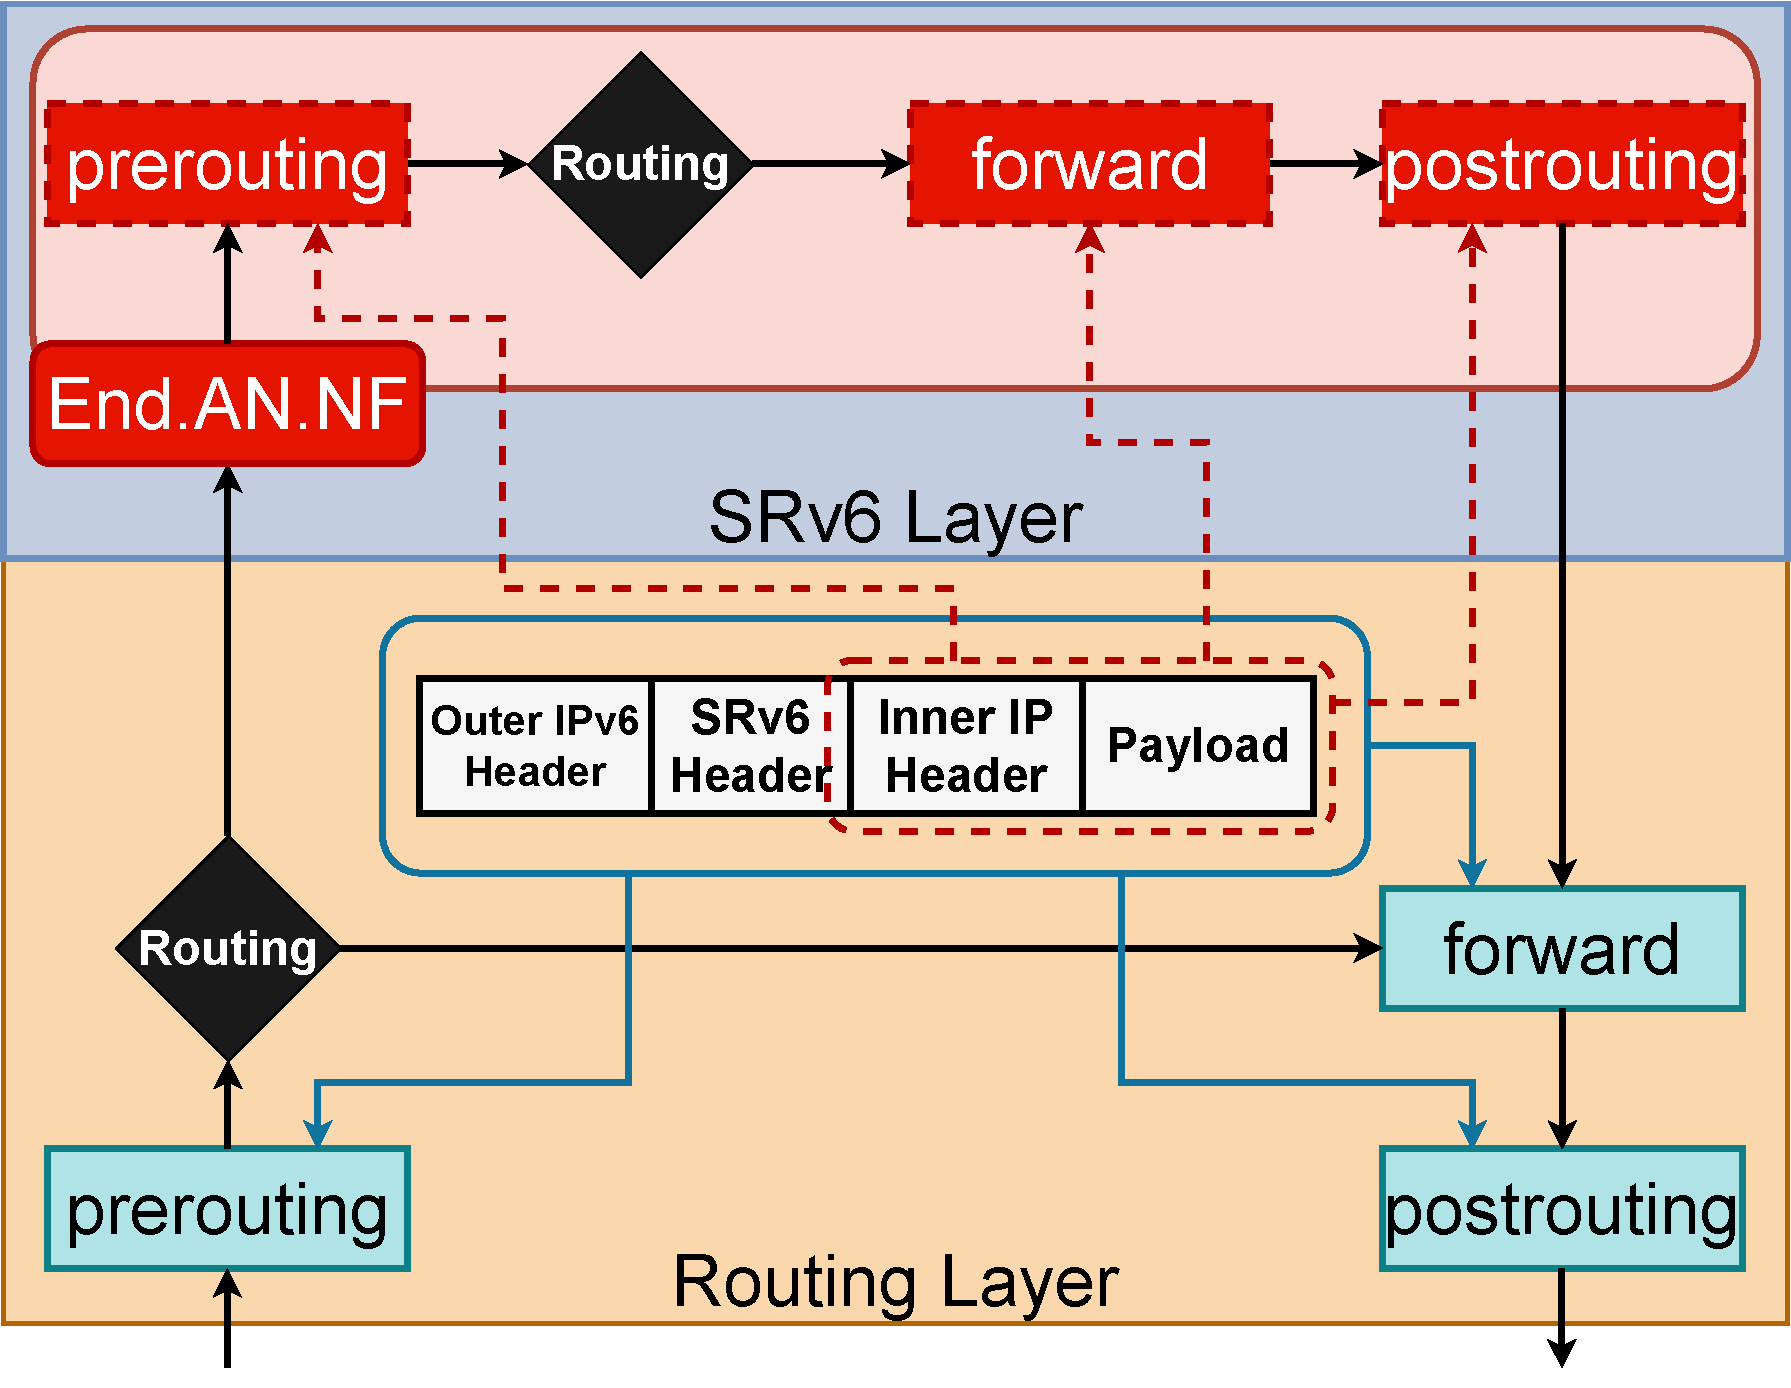
\includegraphics[
      width=0.95\linewidth,
      keepaspectratio=true
    ]{img/End-AN-NF-hooks.pdf}
    \caption{\texttt{End.AN.NF} applies three netfilter hook points, prerouting, forward, and postrouting, to inner packets encapsulated in SRv6.}
    \label{fig:hooks}
  \end{figure}
  
  \begin{algorithm*}[t]
    \caption{Pseudo code of passing a packet to a netfilter hook point in \texttt{End.AN.NF}}
    \small
    \label{alg:end-an-nf}
    \begin{algorithmic}[1]
      \if 0
      \Function {Process\_End.AN.NF}{$packet$}
      \State Call function \textbf{Pass\_to\_Hook} with following args: ($packet$, prerouting)
      \State Decrement segleft by 1
      \State Rewrite destination address based on the SID list and segleft, in the SID of the $packet$
      \State Lookup next hop in th routing table entry for rewrite new destination address
      \State Call function \textbf{Pass\_to\_Hook} with following args: ($packet$, forward)
      \State Call function \textbf{Pass\_to\_Hook} with following args: ($packet$, postrouting)
      \EndFunction
      \fi
      % \Function {Pass\_to\_Hook}{$packet$, $hook\_point$}
      \Function {PassPacketToHook}{$packet$}
      \If {the length of $ARG$ is specified for this \texttt{End.AN.NF} SID}
      \State Extract the $ARG$ value from the destination address of outer SRH
      \State Mark the $ARG$ value on the packet buffer $packet$
      \EndIf
      \State Switch the head of packet buffer $packet$ from the outer SRH to the inner packet
      \State Pass $packet$ to a netfilter hook
      \State Switch the head of packet buffer $packet$ from the inner packet to the outer SRH
      \EndFunction
    \end{algorithmic}
  \end{algorithm*}
  
  \begin{figure*}[t]
    \centering
    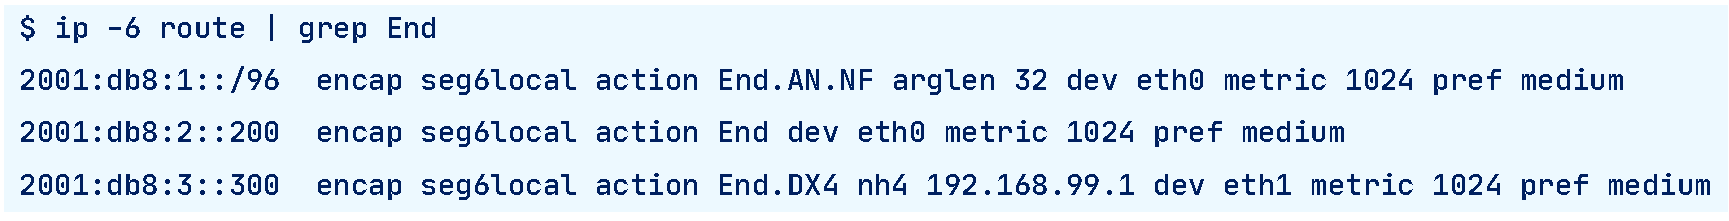
\includegraphics[width=0.95\linewidth]{img/End-FW-show-route.pdf}
    \caption{The modified Linux kernel treats an \texttt{End.AN.NF} SID as an IPv6 routing table entry. We can manage the \texttt{End.AN.NF} routes with the existing tools such as iproute2.}
    \label{fig:show-route}
  \end{figure*}
\chapter{評価}
\label{chap:evaluation}

我々が実装した End.AN.NF の性能を評価するために,3つの実験を行った.
本章では,3つの計測実験で得られた結果から,提案手法が実用上十分なスループット性能を持っているか,及び実用的なレイテンシに収まっているのかを確認するために Linux に実装されている既存のパケット転送メカニズムと比較し評価する.
このうち2つはスループットについて,もう1つはレイテンシについて焦点を当てたものである.
最初の実験では,パケットサイズに基づくスループットを計測し,2つ目の実験では,netfilter ベースのアプリケーションにおけるフィルタールール数を増加させた際のスループットの変化を評価した.
3つ目の実験では,異なるパケット転送メカニズムに関連するレイテンシを計測した.
また,計測用パケットの送信に利用したトラフィックジェネレータ,及び評価の際に考慮したレシーブサイドスケジューリングについても解説する.
\section{計測の概要と予想}
\label{sec:eval-prediction}
End.AN.NF の性能を,3つの転送メカニズムと比較する.
比較対象は,End,End.DT4 と H.Encaps の組み合わせ,及び IPv4 である.
IPv4 は Linux のパケットフォワーディング性能におけるベースラインとして参照する.
図~\ref*{fig:hooks}に示すように,End.AN.NF が動作する場合,受信パケットは End と比較して2倍の数のフックポイントを通過する.
したがって,End.AN.NF の性能は End に劣ることが予想される.
一方で,End.AN.NF の性能は End.DT4 と H.Encaps の組み合わせよりも高いと予想される.
SRv6 でカプセル化されたパケットに netfilter のルールを適用する場合,バニラ Linux カーネルでの実用的なアプローチは End.DT4 と H.Encaps の組み合わせである.
しかし,バニラ Linux カーネルには SRv6 でカプセル化された状態の内部パケットに対して netfilter を適用する手法が実装されていない.
よって,パケットを一度カプセル化解除し,再度カプセル化する必要がある.
End.DT4 によってデカプセル化されたパケットは IPv4 パケットとして netfilter のフックポイントを通過し,H.Encaps は新しい SRH を格納する.
この方法では End.DT4 がパケットをデカプセル化し,その後 H.Encaps がパケットを再度カプセル化するため,オーバーヘッドが発生する.
したがって,このオーバーヘッドが性能の低下につながることが予想される.

3つの実験はすべて同じ構成,同じ環境で行った.
100Gbps のリンクで直結された2台のマシンを用意した.
2台のマシンは同一仕様で,CPU には Intel(R) Xeon(R) Silver 4310 12コア x2,メモリは 64GB DDR4-2666,NIC には Intel E810 100Gbps を搭載している.
CPU のハイパースレッディング機能は無効に設定した.
1台はトラフィック・ジェネレータとして,もう1台は SUT (System Under Test) として使用する.
トラフィック生成マシンには Ubuntu 22.04 と TRex~\cite{trex} をインストールし,テストトラフィックの生成に使用した.
一方,SUT マシンにはカスタマイズした Linux カーネル 5.15.106 をインストールし,End.AN.NF と,End.AN.NF の SID を設定するために独自に拡張した iproute2 コマンドを実装した.
また,2台のマシン間のリンクには2つの VLAN を設定し,テストトラフィックを送信するためのリンクと End.AN.NF 動作後に送信されるトラフィックが論理的に別のリンクになるようにした.


\section{TRex}
\label{sec:trex}
\textbf{[TRex について解説する]}

\section{レシーブサイドスケジューリング}
\label{sec:rss}
\textbf{[RSS について解説する]}

\section{パケットサイズ毎のスループット性能}
\label{sec:eval.thru-size}
End.AN.NF,End,IPv4,及び End.DT4 と H.Encaps の組み合わせについて,パケットサイズを増加させながらスループットを測定した.
この実験により,各パケット転送メカニズムにおけるパケットサイズによるスループットの変化が明らかになった.
この実験では,netfilter のルールは使用しなかった.
netfilter のフックポイントは通過するものの,実際に適用されるルールを何も定義せずに計測を行った.
End.AN.NF の,End に対するスループットの低下,及び End.DT4 と H.Encaps の組み合わせに対する性能の向上を評価した.

\subsection{計測内容}
\label{ssec:thru-size.summary}
トラフィック生成マシンで TRex によって生成されたトラフィックを,最小パケット長 126 バイトから最大パケット長 1518 バイトまでパケットサイズを変化させ,SUT マシンに送信した.
測定時のパケット長は次のように計算した: $l=174n+126$.
ここで $l$ はパケット長,$n$ は測定回数である.
$n=0$ から $n=10$ まで,合計10回の測定を行った.

最小パケット長として 126 バイトを選択した理由は,SID リストの長さが 2 である際のタグ付き VLAN を持つ UDP パケットの最小長が 126 バイトだからである.
End.AN.NF は,パケットの segleft をデクリメントするため,SID リスト長は少なくとも 2 である必要がある.
これは SID リストの長さが 1 の場合,segleft は 0 から始まり,End.AN.NF でデクリメントすると負の値になってしまうからである.
一方,End.DT4 は,segleft が 0 であることを必要とする.
End.DT4 は SRv6 ネットワークの終点で SRH をでカプセル化するビヘイビアである.
つまり,End.DT4 が動作するのは SID リストによって指定された最後のノードであるため,segleft はそれ以上デクリメントできない 0 である必要がある.
そこで,End.DT4 と H.Encaps の組み合わせの測定では,TRex は SID リスト長が 2 のパケットを生成し,segleft を 0 に設定した.
また,レシーブサイドスケジューリング (RSS) の仕組みを効果的に使用するため,TRex でパケットを生成する歳に内側の IPv4 パケットの宛先アドレスと送信元アドレスの両方をインクリメントした.
IPv4 パケットの計測の際は,SRv6 パケット長に合わせて UDP ペイロードにダミーデータを埋め込み,最小パケット長が 126 バイトから始まるようにした.
End.DT4 と H.Encaps の組み合わせの計測と同様,RSS を効果的に活用するため,パケット生成時に宛先アドレスと送信元アドレスをインクリメントした.
最大パケット長については,タグ付き VLAN ヘッダを含むイーサフレームの最大サイズが 1518 バイトであることから,今回の測定ではパケットサイズの上限を 1518 バイトに設定した.

\subsection{評価}
\label{ssec:thru-size.eval}
図~\ref{fig:size-thru} に,この実験の結果を示す.
End.AN.NF のスループットは,すべてのパケット長において End と比較して 6\% 以上の低下は見られない.
パケット長が 1518 バイトのとき,End.AN.NF は End と比べた際のスループットの低下が最も少なく,その低下は約 1.7\% である.
対して,パケット長が 478 バイトのとき,End と比較した際の End.AN.NF のスループットの低下は最も大きく,その低下は 約5.6\% である.
パケット長とスループットには相関がなく,大きな変動が見られた.
このスループットの低下は,End.AN.NF のパケットが End のパケットに比べて2倍の netfilter のフックポイントを通過することが原因として挙げられる.
ただし,そのスループット低下のレベルは許容範囲内に留まっている.

End.AN.NF のスループットを End.DT4 と H.Encaps の組み合わせと比較した場合,End.AN.NF は予想通り,パケット長に関係なく一貫して優れた性能を示している.
具体的には,End.AN.NF は End.DT4 と H.Encaps の組み合わせよりも,最大で 26.7\% 高いスループットを達成している.
グラフから,End.AN.NF と End.DT4 と H.Encaps の組み合わせとの間のスループットの差はパケット長の影響を受けていることが読み取れる.
短いパケットでは相対的な性能格差が大きくなり,長いパケットではその差は縮まる.
パケットサイズが小さくなるにつれて,1秒あたりのパケット転送レート (pps) は増加する.
結果として,パケットサイズが小さいほど,パケット転送のオーバーヘッドが顕著になる.

\begin{figure}[t]
    \centering
    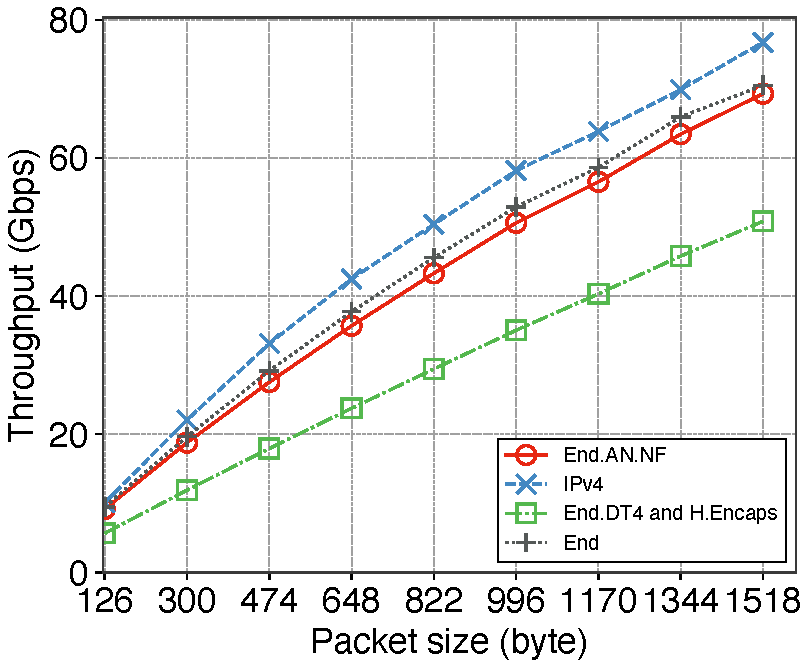
\includegraphics[width=0.95\linewidth]{img/size-throughput.pdf}
    \caption{Throughput per SRv6 End behaviors and IPv4}
    \label{fig:size-thru}
\end{figure}


\section{netfilter にインストールされたルール毎のスループット}
\label{sec:eval.thru-chains}
次に,End.AN.NF,IPv4,および End.DT4 と H.Encaps の組み合わせについて,netfilter にインストールするフィルタールールの数を変更しながらスループットを測定した.
フィルタールールのインストールには,netfilter ベースのアプリケーションとして nftables を使用した.
nftables では,ルールはチェインの集合として表現され,チェインにはベースチェインとレギュラーチェインの2種類がある.
nftables は,他のチェインがレギュラーチェインを参照している場合のみ,レギュラーチェインを使用する.
実験では,チェインの種類ごとにカウントを増やしながらスループットを測定した.
パケット転送メカニズムに関わらず,フィルタールールの追加によりスループットが低下することが予想される.
この実験は,フィルタールールによる各パケット転送メカニズムのスループット低下の特徴を明らかにすることを目的とする.

\subsection{nftables}
\label{ssec:thru-chains.nftables}
\textbf{[nftables について解説する. 特に regular chain と base chain について詳しく記す.]}


\subsection{計測内容}
\label{ssec:thru-chains.summary}
トラフィック生成マシンで TRex が生成したトラフィックを SUT マシンに送信した.
この測定では,パケット長を一貫して 126 バイトに設定した.
パケット長を 126 バイトに設定した理由はセクション~\ref{ssec:thru-size.summary} で説明したものと同じで,SID リスト長が 2 の場合のタグ付き VLAN の UDP パケットの最小長が 126 バイトだからである.

\subsection{評価}
\label{ssec:thru-chains.eval}
図~\ref{fig:rule-thru}は,ベースチェインのルール毎のスループットを示している.
全てのチェインルールがベースチェインのみで構成されるこれらのチェインルールは,nftables のチェインルールの定義の中でも最も性能の出ないルール定義の1つである.
この測定では,netfilter のフォワードフックポイントにフィルタールールを設定した.
netfilter は 1 つのフックポイントに複数のルールを設置できる.
実験を通して,このフックポイントで適用される同一のカスケードルールの数を増加させた.
すべてのパケット転送メカニズムにおいて,スループットはルール数の増加と共に低下する.
ルール数が増加するにつれて,3 つのパケット転送メカニズムすべてのスループットは約 0.4 Mbps に収束する.
End.AN.NF と IPv4 のスループットを比較すると,スループット低下における顕著な特性の違いは見られず,End.AN.NF は IPv4 に対して大きく劣るスループット低下特性を示さない.
一貫して,End.AN.NF は End.DT4 と H.Encaps の組み合わせのスループットを上回る.
しかし,このスループットの差はルール数が増えるにつれて縮小し,128 ルールではわずか 9\% の差まで減少した.
よって,レギュラーチェインのルール数が増加するにつれて,End.AN.NF の End.DT4 と H.Encaps の組み合わせに対する優位性は低下すると言える.

図~\ref{fig:reg-thru}は,ベースチェインのルール数毎のスループットを示している.
注目すべき点は,ルール数を増加させてもスループットの低下が認めれず,かつ End.AN.NF が一貫して End.DT4 と H.Encaps の組み合わせを上回っていることである.
レギュラーチェインのフィルタールールは,ベースチェインで測定した際と同じ構成である.
通過するパケットをすべてアクセプトするルールが定義されており,一度受け入れるルールが適用されたあとも,事前に決めた回数同じ内容のルールが適用され続ける.
しかし,レギュラーチェインのみから成るこのようなルール構成では,定義されたレギュラーチェインが他のチェインから参照されていないため,実際にはルールがパケットへ適用されることはない.
その結果,パケットが netfilter のフックポイントを通過する際に実際に適用されるルールの数は変わらない.

\begin{figure}[t]
  \centering
  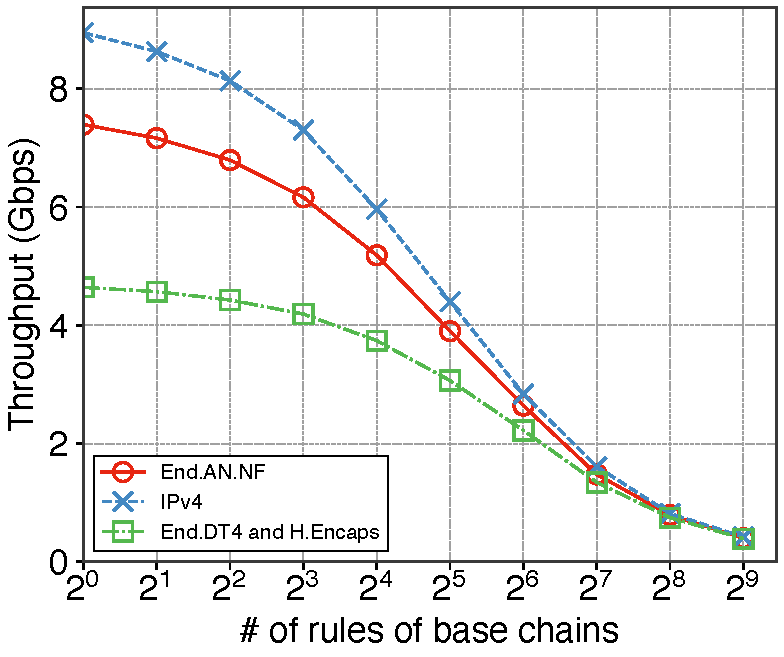
\includegraphics[width=0.95\linewidth]{img/rule-throughput.pdf}
  \caption{Throughput per number of rules of base chains}
  \label{fig:rule-thru}
\end{figure}

\begin{figure}[t]
  \centering
  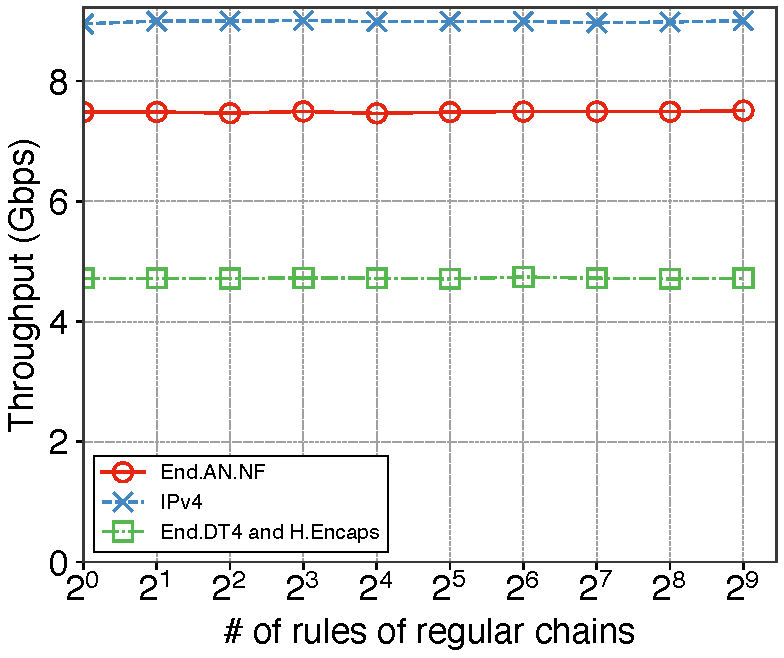
\includegraphics[width=0.95\linewidth]{img/regular-throughput.pdf}
  \caption{Throughput per number of rules of regular chains}
  \label{fig:reg-thru}
\end{figure}

\section{レイテンシ}
\label{sec:eval.rtt}
スループットと同様に End.AN.NF,End,IPv4,及び End.DT4 と H.Encaps の組み合わせについて,レイテンシを測定した.
この計測では特に,End.DT4 と H.Encaps の組み合わせと比較して,End.AN.NF のレイテンシがどれだけ改善されたのか評価することを目的としている.
この評価では,ベースラインとして IPv4 のレイテンシを用いた.

\subsection{計測内容}
\label{ssec:rtt.summary}
スループットと同様に,計測には TRex を使用し,パケット転送のレイテンシを測定した.
TRex はパケットの送受信時間間隔をマイクロ秒単位で測ることが可能である.
今回の測定は,パケット長を 142 バイトに設定した.
142 バイトの内訳について,先頭 126 バイトはセクション~\ref{ssec:thru-size.summary} で説明した通りで,End.AN.NF がの動作要件を満たす最小のパケットとして必要だからである.
追加の 16 バイトは,TRex がよるレイテンシを測定する際に利用するメタデータの埋め込みに使用される.
実験中,トラフィック生成マシンは SUT に対して毎秒 10000 個のパケットを10秒間送信した.
今回のレイテンシ測定では,RSS を無効化するために送信元アドレスと宛先アドレスを変更しなかった.
なぜなら,この規模の pps で RSS を使用してパケットを処理する CPU コアを分散させてしまうと,かえってレイテンシが悪化し,余分なジッタが発生することがあるからである.

\subsection{評価}
\label{ssec:rtt.eval}
計測結果を図\ref{fig:rtt} に示す.
これらのグラフの各データポイントは,100000 回のレイテンシ測定の平均値を表している.
End.AN.NF,End,IPv4 のレイテンシはどれも 16.0 マイクロ秒である.
対照的に,End.DT4 と H.Encaps の組み合わせは 19.0 マイクロ秒のレイテンシである.
マイクロ秒単位での測定では,End.AN.NF のレイテンシは End と IPv4 のレイテンシと一致し,End.DT4 と H.Encaps の組み合わせのレイテンシよりも約 15.8\% 高速であることが分かる.

\begin{figure}[t]
    \centering
    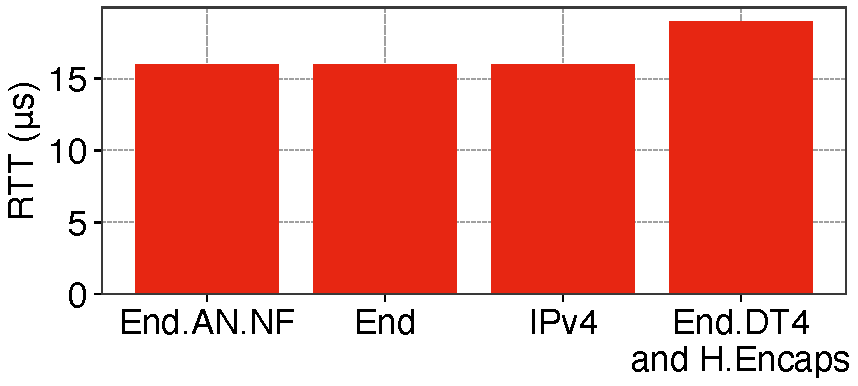
\includegraphics[width=0.95\linewidth]{img/latency.pdf}
    \caption{Latency per SRv6 End behaviors and IPv4}
    \label{fig:rtt}
\end{figure}
\chapter{結論}
\label{chap:conclusion}
\chapter*{謝辞}\markboth{謝辞}{謝辞}
\addcontentsline{toc}{chapter}{謝辞}
\label{thanks}
感謝.

\renewcommand{\thechapter}{\Alph{chapter}}
\setcounter{chapter}{0}
\vspace{-5mm}


\bibliographystyle{unsrt}\pagestyle{plain}
\bibliography{bib/cites}\pagestyle{plain}
\thispagestyle{plain}%bibtex


\end{document}

%%% Local Variables:
%%% mode: japanese-latex
%%% TeX-master: t
%%% End:
